% AER-Article.tex for AEA last revised 22 June 2011
%%\documentclass[AER]{AEA}
\documentclass[12pt,letterpaper]{article}
%%%\usepackage{biblatex}
\usepackage[round]{natbib}
\usepackage{fullpage}
\usepackage{url}
\usepackage{graphicx}
\usepackage{csvsimple}
\usepackage[flushleft]{threeparttable}
\usepackage{amsmath,amssymb}
\usepackage[makeroom]{cancel}
\usepackage[utf8]{inputenc}
\usepackage[english]{babel}
\usepackage[compatibility=false,labelfont=bf]{caption} 
\captionsetup[table]{skip=10pt}
\usepackage{multirow}
\DeclareMathOperator{\E}{\mathbb{E}}
\DeclareMathOperator{\R}{\mathsf{R}}
\DeclareMathOperator{\y}{\mathsf{y}}
\DeclareMathOperator{\pLev}{\pmb{p}}

%Import the natbib package and sets a bibliography  and citation styles
%%\usepackage{natbib}
%%\bibliographystyle{abbrvnat}
%%\setcitestyle{authoryear,open={(},close={)}}
%%%%%% NOTE FROM OVERLEAF: The mathtime package is no longer publicly available nor distributed. We recommend using a different font package e.g. mathptmx if you'd like to use a Times font.
% \usepackage{mathptmx}

% The mathtime package uses a Times font instead of Computer Modern.
% Uncomment the line below if you wish to use the mathtime package:
%\usepackage[cmbold]{mathtime}
% Note that miktex, by default, configures the mathtime package to use commercial fonts
% which you may not have. If you would like to use mathtime but you are seeing error
% messages about missing fonts (mtex.pfb, mtsy.pfb, or rmtmi.pfb) then please see
% the technical support document at http://www.aeaweb.org/templates/technical_support.pdf
% for instructions on fixing this problem.

% Note: you may use either harvard or natbib (but not both) to provide a wider
% variety of citation commands than latex supports natively. See below.

% Uncomment the next line to use the natbib package with bibtex 
%\usepackage{natbib}

% Uncomment the next line to use the harvard package with bibtex
%\usepackage[abbr]{harvard}

% This command determines the leading (vertical space between lines) in draft mode
% with 1.5 corresponding to "double" spacing.
%%\draftSpacing{1.5}
\setlength{\parskip}{0.5em}
\begin{document}

\title{Consumption Dynamics Under Socially Formed Expectations}
%%\shortTitle{Evidence from Value Added Perspective}
\author{Tongli Zhang\thanks{Department of Economics, Johns Hopkins University\newline \hspace*{1.5em} Email: tzhang31@jhu.edu\newline \hspace*{1.5em} I am grateful to Prof. Christopher Carroll for advising my research. I would also like to thank Edmund Crawley, Nicholas Johnson, and Prof. Olivier Jeanne and Prof. Alessandro Rebucci for helpful discussions and comments.}}
\date{\today}
%%\pubMonth{Month}
%%\pubYear{Year}
%%\pubVolume{Vol}
%%\pubIssue{Issue}
%%\JEL{}
%%\Keywords{}

\maketitle
\begin{abstract}
	This paper studies the consumption dynamics when household expectations of future income are affected by other members in his social network. By introducing a social network and the concept of neighborhood into the sticky expectation model, I show that allowing consumers to form their expectations of future income by using their neighbors' information about the macroeconomy increases the variance of aggregate consumption. This is because the social interaction increases the diffusion of the information about productivity shocks, reducing the sluggishness of aggregate consumption. In the model, social interaction also generates a ``group think'' effect: the household who has a high individual productivity also tends to have a higher perception of aggregate productivity, which also increases the variance of aggregate consumption.
\end{abstract}

\section{Introduction}
Empirical evidence suggests that an individual’s consumption is affected by the consumption level of other members in his social network. \cite[]{PeerEvidence} The existing literature explains this effect by incorporating other people's consumption directly into the household utility function. \cite[]{GaliKeep}\cite[]{Veblen1996} The idea is that an individual's utility is not just determined by his absolute consumption level, instead an individuals' utility is also affected by his consumption level relative to other people's consumption.
This paper provides an alternative explanation where other peoples' income and consumption affects the household's consumption decision by affecting the information set of the household. Specifically, I introduce a model where the household does not always observe aggregate productivity; instead the household forms his perception about aggregate productivity by looking at the perceived productivity of other members (we refer to them as neighbors, see Section 2.2 for details) in his social network, and makes his consumption decision based on his perception.
Because the household uses his neighbors' perceptions of the aggregate state to form his own perception, one household's inaccurate perceptions can transmit through the social network, causing the household consumption to collectively deviate from the fundamentals, which may lead to a boom and bust cycle.\par
The model is build upon the sticky expectation model calibrated by \cite{StickyE} to match the quarterly consumption movement. In the original sticky expectation model, an individual's income is determined by the product of aggregate productivity and his individual productivity factor. In each period, both aggregate productivity and individual productivity are subject to permanent and transitory shocks. Further, the household does not always observe the true aggregate productivity. Instead, in each period each household observes the true value of aggregate productivity with some positive probability, at which point he updates his perceptions to be accurate. For the household that does not observe the true aggregate productivity, his information set about the aggregate state stays the same as it was in the last period. So in each period, there is a proportion of households that do not update their information set; this will cause the consumption in aggregate to be sluggish, which can be used to explain the "excessive smoothness" of the consumption in the data \cite[]{EvidenceSlugg}.\par
The major difference between the model in this paper and the original sticky expectation model is that here, in addition to some households updating their perceptions to the true value of true aggregate productivity, some others who do not update fully and accurately are has a probability to update their perceptions of aggregate productivity through their social network. Specifically, in each period, each household has a constant probability $S$ to go to a social gathering, in which case he sets his perception of aggregate productivity to be the average of his neighbors perceived individual productivities (see Section 2.2 for details). The fact that a group of households form their perceptions based on their neighbors' perceived productivities allows the household consumption decision to be affected by his neighbors' perception. Because the household consumption is positively correlated with his perceived income, the consumption of the household who forms his perception from social circle moves in the same direction as his neighbors' average consumption moves.\par
In the model, the household always correctly observes his current income, asset, and consumption level. His perception of aggregate productivity affects his decision by influencing his expectation of future income. This is a deviation from rational expectation theory. In a rational expectation setting where the household always has perfect information about the state variables, there is no room for household's consumption to deviate from the fundamentals. There is good evidence from the survey data suggesting that individuals' expectations of macroeconomic variables such as inflation, and unemployment rate are different from the implication of the rational expectation theory. \cite[]{InflationEvid}\cite[]{SurveyData}
To the best of my knowledge, there is no existing literature on how the household's expectation of future income is impacted by other members in his social network. The most closely related research is done by \cite{Facebook} on the individual's perception of the housing market. They found that an individual's perception of the attractiveness of the housing market was affected by the recent house price experiences of his facebook friends. Individuals whose geographically-distant friends experienced larger recent house price increases consider local property a more attractive investment.
\par
After introducing the model, I studied how the socially formed expectations influence aggregate and individual consumption volatility by simulating a small open economy where households have sticky expectations and are allowed to update their perceptions through social gatherings. I also studied how the variances of aggregate consumption and individual consumption growth change when the size of social network (which is the number of neighbors one household has) changes in such economy.\par
The result shows that when consumers uses their neighbors' perceived productivities to form his own perception of aggregate productivity through social gathering, the variance of individual consumption is higher than the frictionless model where consumers have perfect information about the aggregate state. In both the frictionless model and the original sticky expectation model, the variance of individual consumption is caused by the volatility of perceived income. According to the calibration of \cite{StickyE}, the standard deviation of idiosyncratic shocks is significantly larger than the standard deviation of aggregate shocks, so the variance of perceived income is mostly caused by the idiosyncratic shocks. In the original sticky expectation model, the distortion of the household perception is due to the fact that the non-updating household has outdated perception of the aggregate state, which has very small impact on the variance of individual consumption. In the model where household update his perception through social gathering, because the household can only observe his neighbor's perceived individual productivity which is the product of his neighbors' individual productivity factor and his neighbor's perception of aggregate productivity, the perception of the household who updates his perception in social gathering (we can refer to him as a socially updating household) is distorted in the direction of:
\begin{itemize}
	\item the deviations of his neighbors' individual productivity factors from the average individual productivity factor (equals to 1)
	\item the deviation of their perceived aggregate productivities from the true aggregate productivity.
\end{itemize}
Because the neighbor's individual productivity factor is subject to idiosyncratic shocks, a socially updating household's perception of the aggregate state is influenced by his neighbors' idiosyncratic shocks. Because the standard deviation of idiosyncratic shocks is significantly larger than the standard deviation of aggregate shocks, the household's perception of aggregate productivity is much more volatile than the true aggregate productivity. The household's volatile perception about the aggregate state makes the variance of individual consumption in this model higher than results from the frictionless model and the original sticky expectation model. When the size of social network increases, neighbors' idiosyncratic shocks cancel out each other when the socially updating household takes the average of his neighbors' perceptions, the household perception is less affected by his neighbors' idiosyncratic shocks, the variance of individual consumption converges towards the result of the frictionless model. (See Section 5.3 for detail)
\par
The simulation result also shows that allowing households to update their perceptions through the social channel increases the variance of aggregate consumption compared with the result from the original sticky expectation model. The variance of aggregate consumption in the original sticky expectation model is smaller than the result from the frictionless model because aggregate consumption growth is sluggish in the sticky expectation model. The socially updating mechanism increases the variances of aggregate consumption due to two reasons.\par
First, the socially updating mechanism reduces the sluggishness of the aggregate consumption by giving the household another channel to learn the information about the aggregate state in addition to observing the true state directly. For the socially updating household, there is a chance that some of his neighbors observe the true aggregate state. By setting his perception to be the average of his neighbors' perceived individual productivity, the socially updating household incorporate part of the new aggregate shocks into his perception. This reduces the sluggishness of the sticky expectation model and pull the result towards the frictionless model.\par
Second, the socially updating mechanism allows household perceptions of aggregate productivity to be correlated with their own individual productivity factor. As a result, the idiosyncratic shocks affect the aggregate consumption. In the original sticky expectation model, the household's perception of aggregate productivity is independent from his individual productivity factor. Because there is a large number of households, their individual productivity factors cancel out each other in aggregation; the variance of aggregate consumption is not affected by idiosyncratic shocks. In the model where households update their perceptions through social gathering, this is not true. In this case, the perception of aggregate productivity of the socially updating household is positively correlated with his own individual productivity factor. In this paper, we refer to this phenomenon as ``group think'' because the shocks to the individual productivity factors are shared in the group of socially updating households who are each other's neighbors. The intuition is following: for a socially updating household ``A'', his perception contains his neighbors' perceived individual productivities which are products of each neighbor's individual productivity factor and their perceptions of aggregate productivity. If his neighbor ``B'' also updates perception in social gathering, the neighbor B's perception also contains household A's perception of the aggregate state which includes household B's individual productivity factor. As a result, household B's perception of the aggregate state is positively correlated with his own individual productivity factor. Because their perceptions are mutually dependent, it is also true for household A. When the household perception of aggregate productivity and his individual productivity are positively correlated, the individual productivity factor do not cancel out each other in aggregation, so the aggregate consumption is also affected by idiosyncratic shocks. Because the standard deviation of idiosyncratic shocks are much larger than the standard deviation of aggregate shocks, the variance of aggregate consumption in a model with socially updating consumers are larger than the result from the original sticky expectation model. The impact of ``group think'' decreases as the size of social network increases, so the variance of aggregate consumption decreases when the size of the social network increases.(See Section 5.1 for details)\par
This paper is related with previous literatures about the economic impact of the social network. One group of literature in this area focuses on the influence of social network on macro economy when the topological structure of the network is given. This paper belongs to this group. Research in this group can be traced back to \cite{Granovetter1973} on how interpersonal relations affects the household's information on the job vacancy distribution. Building on the findings of Granovetter, \cite{VacancyNet} developed a model where agents obtain information about job opportunities through their social networks. They showed that the influence of the social network can explain the positive correlation of employment across time and agents, as well as the duration dependency of unemployment. \cite{Stability} introduced the social network into a New Keynesian DSGE model, and studied the influence of social network on macro stability. As far as I know, there is no existing literature studying the impact of the social network on the aggregate consumption. This paper is the first step towards that direction. Another group of literatures study the model with endogenous network formation. One related paper in this group is \cite{ConsumptionManage} where the consumer chooses consumption among a group of substitutable goods and the consumption of each goods has externalities through an endogenously formed network. \cite{EndogNet} showed that the endogenously formed credit network between firms and banks could lead to an avalanche of bankruptcies. This paper is also related (to a less degree) to the micro theory literatures on how the structure of the network influences the diffusion of information through social network. (\cite{MicroSurvey}, \cite{MicroStructure})\par
This paper is also related to literatures on information cascade and herd behavior in finance. The idea is that each individual investor form his perception about the market by looking at other investors' previous behaviors, so one investor's early decision may cause a large group of investors' investment positions to move in the same direction in the next period, resulting in mis-pricing of assets (\cite{HerdOrigin}, \cite{HerdUncertain}). The paper in this area is relevant because the investor in such model makes his investment decision by looking at other investors' behaviors, just as the socially updating consumer in this paper makes his consumption decision by looking at his neighbors. One difference between the social learning in this paper and the social learning in finance literatures is that the finance literature highlights the importance of the investor's early decision because the model is usually sequential. In this paper, all households update their perceptions simultaneously, so the perceptions of household have equal impact across time and agents.\par
The rest of the paper is organized as follows. In Section 2, I present the structure of the social network, and the analytical solution for a toy model to show the intuition of the impact of socially formed perceptions of households. In Section 3, I introduce the full-version model which has more realistic assumptions. After showing the calibration of the model in Section 4, I present the simulation results in Section 5 and show that the intuition we derive from the simplistic toy model still holds in the full-version model. Section 6 is the conclusion.

\section{Solution of A Toy Model}
In this section, I introduce the concept of social learning in the context of the sticky expectation model and show the result of the social learning by using a simple model with quadratic utility. Later, I will show that the result we derive from this simple model holds in a model with more realistic settings.
\subsection{Informational Friction and Sticky Expectation}
The social learning is build on \cite{StickyE} sticky expectation model. Here I briefly introduce the background and the intuition of the sticky expectation. We can start with the classic \cite{Hall1978} random walk model where the household has time separable utility function and geometric time discount rate $\beta$. The household dynamic budget constraint is:
\begin{equation} \label{Toy:DBC}
\mathrm{o}_{t+1}=(\mathrm{o}_{t}-\mathrm{c}_{t})\mathsf{R}+\zeta_{t+1}
\end{equation}
Here $\mathrm{o}_{t}$ is the household total wealth (sum of human and nonhuman wealth) at time period $t$. $\mathsf{R}=1+\mathsf{r}$ is the interest rate factor, $\zeta_{t+1}$ is the shock to total wealth. Each household optimizes the expected life time utility function. In the case there is no informational friction, the first order condition leads to Euler equation:
\begin{equation} \label{Toy:Euler}
\mathrm{u}'(\mathrm{c}_{t})=\mathsf{R}\beta\E_{t}\left[\mathrm{u}'(\mathrm{c}_{t+1})\right]
\end{equation}
Here the unconditional expectation $\E_{t}$ denotes the assumption that the household instantaneously updates all information perfectly in each period, there is no friction in the updating process. Quadratic $\mathrm{u}$ and $\R\beta=1$ imply that the household consumption follows a random walk process:
\begin{equation*}
\E_{t}\left[\Delta\mathrm{c}_{t+1}\right]=0
\end{equation*}
At steady state: $\E_{t}\left[\mathrm{o}_{t+1}\right]=\left(\mathrm{o}_{t}-\mathrm{c}_{t}\right)\R=\mathrm{o}_{t}$. The consumption in the frictionless case is:
\begin{equation*}
\mathrm{c}_{t}=\frac{\mathrm{r}}{\R}\mathrm{o}_{t}
\end{equation*}
\par
Contrast to the frictionless model, in the sticky expectation model, the household does not always update information instantaneously. Instead, in each period, each household has a probability $\Pi$ to update their information about the wealth. A consumer who updates in period $t$ receives the same information as the consumer in the frictionless model does, as the result, he forms the same expectation and makes the same choice. For the consumer who does not update in period $t$, he will behave as if his last period expectation of the wealth is the true wealth. For example, for a consumer who updates in period $t$ and period $t+n$ but not in between, his perception of the wealth $\tilde{\mathsf{o}}$ is:
\begin{equation*}
\tilde{\mathrm{o}}_{t+j}=\E_{t}\left[\mathrm{o}_{t+j}\right]=\mathrm{o}_{t}\text{  }\forall\text{  }1\leq j<n
\end{equation*}
The consumer chooses his consumption according to his perception:
\begin{equation*}
\mathrm{c}_{t+j}=\frac{\mathrm{r}}{\R}\tilde{\mathrm{o}}_{t+j}=\frac{\mathrm{r}}{\R}\mathrm{o}_{t}=\mathrm{c}_{t}\text{  }\forall\text{  }1\leq j<n
\end{equation*}
In an economy populated where there is a continuum of consumers indexed by $i$, with mass 1 and distributed uniformly, aggregate consumption is:
\begin{equation*}
\mathrm{C}_{t}=\int_{0}^{1}\mathrm{c}_{t,i}\mathsf{d}i
\end{equation*}
Whether the consumer at location $i$ update his information in period $t$ is determined by a variable $\pi_{t,i}$ which equals 1 if consumer $i$ updates, equals 0 if he does not update. Because in each period, consumers who update are randomly chosen from the population:
\begin{equation}
\E_{t}\left[\pi_{t+1,i}\right]=\Pi\text{  }\forall\text{  }t\text{ ,}i
\end{equation}
\begin{equation}
\int_{0}^{1}\pi_{t+1,i}\mathsf{d}i=\Pi\text{ }\forall\text{  }t
\end{equation}
Which means there is $\Pi$ fraction of the population that updates each period (we refer to these consumers as news updaters because they observe the true state from the news). The aggregate consumption is the weighted average of per-capita consumptions of updaters and non-updaters:
\begin{equation} \label{Toy:StickyE}
\mathrm{C}_{t+1}=\Pi\mathrm{C}^{\pi}_{t+1}+\left(1-\Pi\right)\underbrace{\mathrm{C}^{\cancel{\pi}}_{t+1}}_{=\mathrm{C}_{t}}
\end{equation}
Here $\mathrm{C}^{\pi}_{t+1}$ is the average per-capita consumption of consumers who update in period $t+1$, $\mathrm{C}^{\cancel{\pi}}_{t+1}$ is the average per-capita consumption of non-updaters which equals to the last period average per-capita consumption of the population. We can show that consumption growth is serial correlated in sticky expectation model (Details of the proof is in Appendix A.1):
\begin{equation} \label{Toy:AggC}
\Delta\mathrm{C}_{t+1}=(1-\Pi)\R\Delta\mathrm{C}_{t}+\Pi\epsilon_{t+1}
\end{equation}
Where $\epsilon_{t+1}$ is mean zero. When $\Pi=1$, the sticky expectation model reduces to the frictionless model where every consumer updates his information in each period. Note at steady state, the variance of aggregate consumption growth in sticky expectation model is:
\begin{eqnarray} \label{Toy:AggVar}
\sigma^{2}_{\Delta\mathrm{C}} & = & (1-\Pi)^{2}\R^{2} \sigma^{2}_{\Delta\mathrm{C}}+\Pi^2\sigma^{2}_{\epsilon}\\
\Rightarrow\sigma^{2}_{\Delta\mathrm{C}} & = & \frac{\Pi^2}{1-(1-\Pi)^{2}\R^{2}}\sigma^{2}_{\epsilon} \nonumber
\end{eqnarray}
We can obtain the variance of aggregate consumption growth in the frictionless model by letting $\Pi=1$:
\begin{equation} \label{Toy:AggFric}
\sigma^{2}_{\Delta\mathrm{C}|frictionless}=\sigma^{2}_{\epsilon}
\end{equation}
From equation (\ref{Toy:AggVar}) and (\ref{Toy:AggFric}), we can show that for almost all $\Pi\in(0,1)$, $\sigma^{2}_{\Delta\mathrm{C}|stickyE}<\sigma^{2}_{\Delta\mathrm{C}|frictionless}$\footnote{This is true $\forall$ $\frac{\R^2-1}{\R^2+1}<\Pi<1$, because $\R=(1+\mathsf{r})\approx1$, $\frac{\R^2-1}{\R^2+1}\approx0$} which means the variance of aggregate consumption from the sticky expectation model is smaller than the variance of aggregate consumption from the frictionless model. We can also prove, $\sigma^{2}_{\Delta\mathrm{C}|stickyE}$ increases as $\Pi$ increase\footnote{This is true $\forall$ $1-\frac{1}{\R^2}<\Pi<1$, because $\R=(1+\mathsf{r})\approx1$, $1-\frac{1}{\R^2}\approx0$}, which implies that the variance of aggregate consumption from sticky expectation model increases as the probability of updating increases. The intuition is that in the sticky expectation model, there are a group of consumers that do not change their consumption in each period which makes the aggregate consumption growth sluggish, resulting in smaller variance of $\Delta\mathrm{C}$ compares with the frictionless model. When the probability of updating increases, the fraction of consumers who do not change their consumptions decreases, which reduces the sluggishness of the aggregate consumption growth, so the variance of aggregate consumption growth is higher.
\subsection{Social Network and Social Learning}
Based on the sticky expectation framework, I introduce the concept of the social network and social learning into the model. In order to capture the intuition behind the influence of the social network while keeping the model as close to the original sticky expectation model as possible, here the structure of the social network is simply a circle, and every household takes the the social network as given. Specifically, assume there are $N$ number of consumers in total.\footnote{Here I use the discrete number of consumers to illustrate the concept of neighborhood. Using a continuum of agents does not change the result,  see details in Appendix A.2} Consumers sit in a circle and are numbered clockwise from 0 to $N$. For any given agent $i$, and the given size of neighborhood $n$, we define neighbors of the agent $i$ as the nearest $n$ agents from agent $i$ on both (clockwise and counter-clockwise) sides. Figure \ref{figure:social_network} shows examples of $n=1$ and $n=2$.
\begin{figure}[h]
	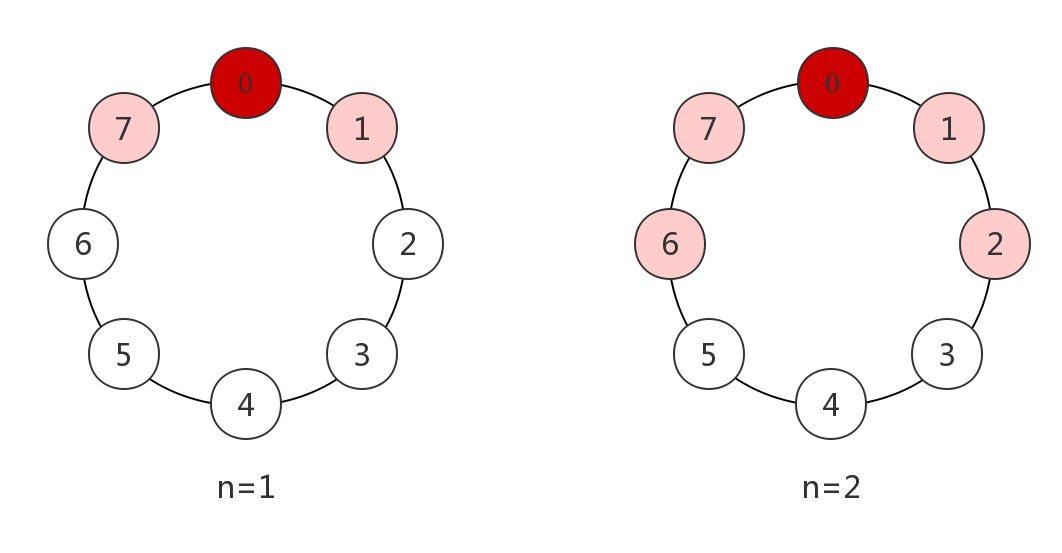
\includegraphics[scale=0.25]{Social_Network.png}
	\centering
	\caption{Illustration for one agent (dark red) and his neighbors (light red)}
	\label{figure:social_network}
\end{figure}
\par
Given the structure of the social network, each household has a probability of learning from their neighbors in each period. In order to describe the social learning mechanism, we need to specify the shocks to consumers' general wealth. Assume for any consumer $i$, his non-human wealth at the beginning of period t is $\mathrm{b}_{t,i}$ ($\mathrm{b}$ stands for the bank balance). Each consumer receives income $\mathrm{y}_{t}$ at the beginning of each period, $\mathrm{y}_{t}$ is subject to aggregate permanent and transitory shocks:
\begin{eqnarray} \label{Toy:Income}
\mathrm{y}_{t+1}=\mathsf{p}_{t+1}\Theta_{t+1}\\
\mathsf{p}_{t+1}=\mathsf{p}_{t}\Psi_{t+1}
\end{eqnarray}
Here $p_{t}$ is the permanent income, transitory shocks $\Theta_{t+1}$ and permanent shocks $\Psi_{t+1}$ are mean 1 i.i.d log-normal processes. So the wealth of consumer $i$ at time period $t$ is:
\begin{equation}
\mathrm{o}_{t,i}=\mathrm{b}_{t,i}+\mathrm{h}_{t}
\end{equation}
Here $\mathrm{b}_{t,i}$ is the non-humane wealth. Human wealth $\mathrm{h}_{t}$ is:
\begin{eqnarray}
\mathrm{h}_{t} & = & \mathrm{y}_{t}+\frac{\E_{t}[\mathrm{y}_{t+1}]}{\mathsf{R}}+\frac{\E_{t}[\mathrm{y}_{t+2}]}{\mathsf{R}^2}+\frac{\E_{t}[\mathrm{y}_{t+3}]}{\mathsf{R}^3}+\cdots\\
& = & (\Theta_{t}-1)\mathsf{p}_{t}+\frac{\mathsf{R}}{\mathsf{r}}\mathsf{p}_{t} \nonumber
\end{eqnarray}
The income process is the same for all consumers, so in the frictionless model, consumers make the same consumption choice:
\begin{eqnarray}
\mathrm{c}_{t,i} & = & \frac{\mathsf{r}}{\mathsf{R}}\mathrm{o}_{t}\\
& = & \frac{\mathsf{r}}{\mathsf{R}}\left[\mathrm{b}_{t,i}+\mathrm{h}_{t}\right]\\ \nonumber
& = & \frac{\mathsf{r}}{\mathsf{R}}\left[\mathrm{b}_{t,i}+(\Theta-1)\mathsf{p}_{t}\right]+\mathsf{p}_{t} \nonumber
\end{eqnarray}
\par
Because the consumer always observes his current bank balance and income, his perception of the wealth is determined by his perception of the permanent income which affects his expectation of future income. Following the original sticky expectation model, we assume the consumer does not always observe the permanent income, instead in each period $t$ each consumer $i$ has a probability $\Pi$ to observe the true permanent income from the news in which case he updates his perception to be the true value: $\tilde{\mathsf{p}}_{t,i}=\mathsf{p}_{t}$ (we refer it as updating to the news, tilde denotes the consumer' perception). In addition, in each period $t$, each consumer also has a probability $S$ to go to a social gathering in which case he takes the average of his neighbors' perceived permanent income to be his own perception of the permanent income\footnote{Here I use the discrete settings to illustrate the updating mechanism. Using a continuum of agents does not change the result,  see details in Appendix A.2}:
\begin{eqnarray} \label{Toy:SocialUpdating}
\tilde{\mathsf{p}}_{t,i}=\frac{1}{2n}\sum\limits_{j=-n,j\neq 0}^n \tilde{\mathsf{p}}_{t,i+j}
\end{eqnarray}
Whether the consumer at location $i$ goes to the social gathering is controlled by a variable $s_{t,i}$ which equals 1 when the consumer $i$ goes to social gathering, equals 0 if he does not. If both $\pi_{t,i}$ and $s_{t,i}$ equal to 1, observing the true permanent income dominates, the consumer will update his perception to be the true value. The updating rule can be summed up as:
\begin{eqnarray}
\begin{cases}
\pi_{t,i}=1  & \text{updating to the news}\\
\pi_{t,i}=0\text{ and }s_{t,i}=1 & \text{updating to the neighbors' average}\\
\pi_{t,i}=0\text{ and }s_{t,i}=0 & \text{not updating}
\end{cases}
\end{eqnarray}
Because consumers that update to the news and to the average perception of their neighbors are chosen randomly from the population, and
\begin{equation}
\E_{t}\left[s_{t+1,i}\right]=S\text{  }\forall\text{  }t\text{ ,}i
\end{equation}
The proportion of consumers that update their perceptions through social gathering (we refer to them as social updaters) in each period is:
\begin{equation}
\int_{0}^{1}(1-\pi_{t+1,i})s_{t+1,i}\mathsf{d}i=(1-\Pi)S\text{  }\forall\text{  }t
\end{equation}
The aggregate consumption is the weighted average of per-capita consumptions of news updaters, social updaters, and non-updaters:
\begin{equation} \label{Toy:Social}
\mathrm{C}_{t+1}=\Pi\mathrm{C}^{\pi}_{t+1}+\left(1-\Pi\right)S\mathrm{C}_{t+1}^{\cancel{\pi},s}+\left(1-\Pi\right)\left(1-S\right)\underbrace{\mathrm{C}^{\cancel{\pi},\cancel{s}}_{t+1}}_{=\mathrm{C}_{t}}
\end{equation}
Here $\mathrm{C}^{\pi}_{t+1}$ is the average per-capita consumption of news updaters, $\mathrm{C}_{t+1}^{\cancel{\pi},s}$ is the average per-capita consumption of social updaters, $\mathrm{C}^{\cancel{\pi},\cancel{s}}_{t+1}$ is the per-capita consumption of non-updaters.
\par
To understand the impact of the social learning process on aggregate consumption dynamic, we can start with an extreme case where $n=\frac{N}{2}$ which means that each consumer's neighborhood includes the entire population. (Note each consumer's neighborhood contains $n$ consumers on both sides) In this case, the socially updating consumer's perception of the permanent income will be the average perception of the entire population. Because consumption is linear in permanent income, the average per-capita consumption of socially updating consumer will equal to the average per-capita consumption of the population:
\begin{equation} \label{Toy:Ninfty}
\mathrm{C}_{t+1}^{\cancel{\pi},s}=\mathrm{C}_{t+1}
\end{equation}
Here the population is normalized to 1, the aggregate consumption is equal to average per-capita consumption of the population. We can derive the dynamic of aggregate consumption from equation (\ref{Toy:Social}) and (\ref{Toy:Ninfty}):
\begin{eqnarray} \label{Toy:Equiv}
\mathrm{C}_{t+1} & = & \Pi\mathrm{C}^{\pi}_{t+1}+\left(1-\Pi\right)S\mathrm{C}_{t+1}+\left(1-\Pi\right)\left(1-S\right)\mathrm{C}_{t} \nonumber\\ \nonumber
\\
\Rightarrow\mathrm{C}_{t+1} & = & \underbrace{\frac{\Pi}{1-\left(1-\Pi\right)S}}_{=\tilde{\Pi}}\mathrm{C}^{\pi}_{t+1}+\underbrace{\frac{\left(1-\Pi\right)\left(1-S\right)}{1-\left(1-\Pi\right)S}}_{=1-\tilde{\Pi}}\mathrm{C}_{t}
\end{eqnarray}
Compare equation (\ref{Toy:Equiv}) with equation (\ref{Toy:StickyE}), we can see that the social learning model is equivalent to a standard sticky expectation model with a modified probability of updating to the truth:  $\tilde{\Pi}=\frac{\Pi}{1-\left(1-\Pi\right)S}\geq\Pi$. Replacing $\Pi$ with $\tilde{\Pi}$ in equation (\ref{Toy:AggVar}) and (\ref{Toy:AggFric}), we can show that the variance of aggregate consumption from the social learning model $\sigma^{2}_{\Delta\mathrm{C}|social}$ satisfies:
\begin{eqnarray} \label{Toy:VarC}
\sigma^{2}_{\Delta\mathrm{C}|stickyE}&<\sigma^{2}_{\Delta\mathrm{C}|social}<&\sigma^{2}_{\Delta\mathrm{C}|frictionless}\text{  }\forall\text{  }0<S<1
\end{eqnarray}
\begin{eqnarray}
\frac{\mathsf{d}(\sigma^{2}_{\Delta\mathrm{C}|stickyE})}{\mathsf{d}S} & > & 0
\end{eqnarray}
The model reduces to the original sticky expectation model when the probability of social learning $S=0$; and to the frictionless model when $S=1$. The intuition is that social gathering gives the consumer a second channel to receive the new information because some neighbors of the consumer are news updaters. The socially updating consumer will adjust his consumption towards the true permanent income, this reduces the sluggishness of aggregate consumption. As a result, the variance of aggregate consumption is higher in social learning model than in the original sticky expectation model.
\section{Real Model}
The discussion in section 2 reveals that consumers learning from neighbors improves the information updating, reducing the sluggishness of aggregate consumption. The model in Section 2 has several simplified assumptions. Introducing the more realistic assumptions could potentially change the conclusion. Specifically, the model in Section 2 assumes every household has the same income process which is determined by aggregate productivity while a more realistic setting would allow the income of consumer to be determined by both individual and aggregate factors. In addition, a standard assumption of utility function in the literatures is constant relative risk averse (CRRA) utility instead of quadratic utility we use in Section 2. Also in Section 2, we only discuss the extreme case when the consumer's neighborhood contains the entire population, a smaller size of neighborhood may change the impact of the social network. In this section, I present a model with CRRA utility, heterogeneous household income trajectories, and a social network with a small size of neighborhood. 
\subsection{General Assumption}
The model is build upon \cite{StickyE} sticky expectation model, most of the general assumptions are the same as the original sticky expectation model. Here I briefly introduce these assumptions. In the model, there is a small open economy populated by a continuum of agents with their mass normalized to be one. All agents sit in a circle, and they are numbered clockwise. Each agent maximizes his expected life-time utility. The agent has CRRA utility function and discounts his future utility flows by time preference factor $\beta$. Output of the economy is determined by the Cobb-Douglass production function:
\begin{eqnarray}
\pmb{\mathrm{Y}}_{t}=\pmb{\mathrm{K}}_{t}^{\alpha}\pmb{\mathrm{L}}_{t}^{1-\alpha}
\end{eqnarray}
Here $\pmb{\mathrm{K}}_{t}$ is the capital level which depreciates at rate $\delta$ immediately after producing output. $\pmb{\mathrm{L}}_{t}$ is the aggregate effective labor. Since the population is normalized to be one, the aggregate effective labor $\pmb{\mathrm{L}}_{t}$ is determined by the productivity level. Aggregate productivity includes a transitory component and a permanent component:
\begin{eqnarray}
\pmb{\mathrm{L}}_{t}=\Theta_{t}P_{t}
\end{eqnarray}
Here transitory shocks $\Theta_{t}$ is mean one i.i.d. The aggregate permanent productivity $P_{t}$ grows by factor $\Phi_{t}$, subject to aggregate permanent shocks $\Psi_{t}$:
\begin{eqnarray}
P_{t+1}=\Phi_{t+1}P_{t}\Psi_{t+1}
\end{eqnarray}
$\E_{t}\left[\Psi_{t+j}\right]$=1 $\forall$ $j>0$. The growth rate of aggregate permanent productivity $\Phi_{t}$ follows a bounded random walk which initially was introduced to capture the fact that productivity growth rate changes substantially overtime\footnote{See Section 4.1.1 in \cite{StickyE} for details}:
\begin{eqnarray}
\text{Prob}(\Phi_{t+1}=\Phi_{k}|\Phi_{t}=\Phi_{j})=\Xi_{k,j}
\end{eqnarray}
Each household $i$ has an individual productivity factor $p_{t,i}$, which is subject to idiosyncratic permanent shocks $\psi_{t}$:
\begin{eqnarray} \label{Ind_p}
p_{t+1}=p_{t}\psi_{t+1,i}
\end{eqnarray}
The idiosyncratic permanent shocks are mean one and i.i.d across time and agents. As a result, in each period, the average individual productivity factor of the population $\int_{0}^{1}p_{t,i}\mathsf{d}i=1$. Each household supply one unit of labor, his contribution to effective labor equals to:
\begin{eqnarray}
\pmb{\ell}_{t,i}= \overbrace{\theta_{t,i}\Theta_{t}}^{\equiv\,\pmb{\theta}_{t,i}}\underbrace{{p}_{t,i} {P}_{t}}_{\equiv\,\pLev_{t,i}}
\end{eqnarray}
Here idiosyncratic transitory shocks $\theta_{t}$ are mean one i.i.d. $\theta$ has minimum possible value 0 to represent an unemployment spell, which happens with probability $\wp$. The risk of becoming unemployed impose a natural borrowing constraint at zero on consumers. In aggregate, the effective labor is:
\begin{eqnarray}
\pmb{\mathrm{L}}_{t}=\int_{0}^{1}\pmb{\ell}_{t,i}=\pmb{\theta}_{t,i}\pLev_{t,i}\text{d}i=\Theta_{t}P_{t}
\end{eqnarray}
\par
For infinitely lived households, his individual productivity factor would spread out infinitely because shocks accumulate over time. In order to avoid this inconvenience, in the model, the household is set to be \cite{blanchardFinite} ``perpetual youth'' consumer. Each agent faces a constant probability of death $\mathsf{D}$ between period. When an agent dies, he is immediately replaced by an unrelated newborn agent who takes the same location on the number circle\footnote{Even though the newborn agent inherites the same location from the dying agent, they are not related. The newborn agent's utility does not enters into the dying agent value function, nor does the newborn agent inherite the dying agent's asset}. The death event of agent $i$ at time period $t$ is controlled by a binary variable $\mathsf{d}_{t,i}$, which equals $1$ if the agent $i$ dies between period $t$ and period $t+1$, or equals $0$ if he survives. The probability of death is identical among agents, so the fraction of population that dies is the same in each period.
\begin{eqnarray}
\int_{0}^{1}\mathsf{d}_{t+1,i}\text{d}i=\E_{t}\left[\mathsf{d}_{t+1,i}\right]= \mathsf{D}
\end{eqnarray}
Newborn agents has the average individual productivity factor of the population which is 1, so the transition of equation (\ref{Ind_p}) can be extended to:
\begin{eqnarray}
p_{t+1,i}=
\begin{cases}
p_{t}\psi_{t+1,i}  & \text{if }\mathsf{d_{t+1,i}}=0\\
1 & \text{if }\mathsf{d_{t+1,i}}=1
\end{cases}
\end{eqnarray}
One primary state variable of the household is his market resource which contains his current period labor income, and total resources that comes from his capital stock (including the capital income of this period and the capital itself):
\begin{eqnarray}
\pmb{\mathrm{m}}_{t,i}=\underbrace{\mathsf{W}_{t}\pmb{\ell}_{t,i}}_{\equiv \pmb{\mathsf{y}}_{t,i}}+\underbrace{\mathcal{R}_{t}}_{1+\mathsf{r}_{t}-\delta}\pmb{\mathrm{k}}_{t,i}
\end{eqnarray}
Here $\pmb{\mathrm{m}}_{t,i}$ is the market resource of agent $i$ at period $t$. $\mathsf{W}_{t}$ is the wage rate for each effective labor. $\pmb{\mathrm{y}}_{t,i}$ is his labor income. $\mathcal{R}_{t}$ is the effective interest rate which is the return of capital after adjusting for depreciation. $\pmb{\mathrm{k}}_{t,i}$ is the capital stock owned by agent $i$ at the beginning of period $t$. The "asset" of the household $\pmb{\mathrm{a}}_{t,i}$ is defined as agent $i$'s market resources at the end of period $t$:
\begin{eqnarray}
\pmb{\mathrm{a}}_{t,i}=\pmb{\mathrm{m}}_{t,i}-\pmb{\mathrm{c}}_{t,i}
\end{eqnarray}
Upon death, the asset of the dying agent is distributed to the surviving agents in proportion to their existing asset, the capital stock of next period evolves according to:
\begin{eqnarray}
\pmb{\mathrm{k}}_{t+1,i}=
\begin{cases}
\frac{\pmb{\mathrm{a}}_{t,i}}{\cancel{\mathsf{D}}}  & \text{if }\mathsf{d_{t+1,i}}=0\\
0 & \text{if }\mathsf{d_{t+1,i}}=1
\end{cases}
\end{eqnarray}
The first row shows that the surviving agent's asset is higher due to the Blanchardian insurance scheme described above. Here $\cancel{\mathsf{D}}=1-\mathsf{D}$
\par
The aggregate capital stock can be obtained as the integral of the individual capital stock across agents:
\begin{eqnarray}
\pmb{\mathrm{K}}_{t}=\int_{0}^{1}\pmb{\mathrm{k}}_{t+1,i}\text{d}i=\int_{0}^{1}\frac{\pmb{\mathrm{a}}_{t-1,i}}{\cancel{\mathsf{D}}}\mathsf{d}_{t,i}\text{d}i=\pmb{\mathrm{A}}_{t-1}
\end{eqnarray} 
The aggregate market resource can be obtained by adding up the market resource of newborn agents and the market resource of surviving agents:
\begin{eqnarray}
\pmb{\mathrm{M}}_{t} & = & (\pmb{\mathrm{A}}_{t-1}\mathcal{R}_{t}\big/\cancel{\mathsf{D}}+\Theta_{t}P_{t}\mathsf{W}_{t})\cancel{\mathsf{D}}+\Theta_{t}P_{t}\mathsf{W}_{t}\mathsf{D}\\
& = & \pmb{\mathrm{A}}_{t-1}\mathcal{R}_{t}+\Theta_{t}P_{t}\mathsf{W}_{t} \nonumber\\
& = & \pmb{\mathrm{K}}_{t}\mathcal{R}_{t}+\pmb{\mathrm{L}}_{t}\mathsf{W}_{t} \nonumber
\end{eqnarray}
\subsection{Solution of the Frictionless Model}
Each household maximizes his expected life-time value utility:
\begin{equation} \label{Bellman}
\mathrm{v}(\pmb{\mathrm{m}}_{t,i},p_{t,i},P_{t},\Phi_t) = \max_{\pmb{\mathrm{c}}_{t,i}} \left\{\mathrm{u}(\pmb{\mathrm{c}}_{t,i}) + \beta \mathbb{E}_{t}\big[(1-\mathsf{d}_{t,i})\mathrm{v}(\pmb{\mathrm{m}}_{t+1,i},p_{t+1,i},P_{t+1},\Phi_{t+1})\big]\right\}
\end{equation}
The problem can be simplified by dividing every part of equation (\ref{Bellman}) with $\pmb{p}_{t,i}=p_{t,i}P_{t}$. Let non-bold letters $\mathrm{m}_{t,i}$, $\mathrm{c}_{t,i}$, $\mathrm{a}_{t,i}$, $\mathrm{k}_{t,i}$ represent the normalized variables. (for example: $\mathrm{m}_{t,i}=\frac{\pmb{\mathrm{m}}_{t,i}}{\pmb{p}_{t,i}}$). The normalized problem only has two state variables $\mathrm{m}_{t,i}$ and $\Phi_{t}$
\begin{eqnarray} \label{Normalized}
\mathrm{v}(\mathrm{m}_{t,i},\Phi_{t}) & = &  \max_{\mathrm{c}_{t,i}}\left\{\mathrm{u}(\mathrm{c})+\cancel{\mathsf{D}}\beta\E_{t}\left[\left(\Phi_{t+1}\pmb{\psi}_{t+1,i}\right)^{1-\rho}\mathrm{v}(\mathrm{m}_{t+1,i},\Phi_{t+1})\right]\right\}
\\  & \mbox{s.t.} & \nonumber
\\   \mathrm{a}_{t,i}   & = & \mathrm{m}_{t,i} - \mathrm{c}_{t,i}, \nonumber
\\   \mathrm{k}_{t+1,i} & = & \mathrm{a}_{t,i} /( \cancel{\mathsf{D}} \Phi_{t+1} \pmb{\psi}_{t+1,i} ),  \nonumber
\\   \mathrm{m}_{t+1,i} & = & \mathcal{R} \mathrm{k}_{t+1,i} + \mathsf{W}\pmb{\theta}_{t+1,i}.  \nonumber
\end{eqnarray}
Here $\pmb{\psi}_{t,i}=\psi_{t,i}\Psi_{t}$, $\pmb{\theta}_{t,i}=\theta_{t,i}\Theta_{t}$. Interest rate $\mathcal{R}$ and wage rate per effective labor $\mathsf{W}$ are fixed over time for small open economy. Defining $\mathsf{R}=\mathcal{R}/\cancel{\mathsf{D}}$, the existence of the solution for the model requires growth impatience condition\footnote{See \cite{BufferTheory} for details}:
\begin{eqnarray}
\mathsf{R}\beta\E\left[\pmb{\psi}^{-\rho}\right]<1
\end{eqnarray}
The solution of the normalized problem represented by equation (\ref{Normalized}) is normalized consumption function $\mathrm{c}(\mathrm{m},\Phi)$. We can obtain the household consumption level by multiplying $\mathrm{c}$ with $\pmb{p}$:
\begin{eqnarray}
\pmb{\mathrm{c}}_{t,i}=\pmb{p}_{t,i}\mathrm{c}(\mathrm{m}_{t,i},\Phi_{t})
\end{eqnarray}
Because the consumption function is linear in permanent income, this is also the solution for the unnormalized problem:
\begin{eqnarray} \label{ConsumptionPolicy}
\pmb{\mathrm{c}}_{t,i}=\hat{\pmb{\mathrm{c}}}(\pmb{\mathrm{m}}_{t,i},p_{t,i},P_{t},\Phi_{t})
\end{eqnarray}
\subsection{Perceptions and Updating Mechanism}
The solution above applies to the situation where agents always has full information of state variables $(\pmb{\mathrm{m}}_{t,i},p_{t,i},P_{t},\Phi_{t})$. One of the key features of the model is that agents do not always observe aggregate state variables $(P_{t},\Phi_{t})$. Instead in each period, each agent has a probability that he does not observe the true aggregate state variables, in which case he makes decision based on his perception of the aggregate states: $(\tilde{P}_{t,i},\tilde{\Phi}_{t,i})$(Here tilde variables are household perceptions). Like I described in Section 2.1, whether the agent $i$ observes the true aggregate states is controlled by a random variable $\pi_{t,i}$ which equals 1 if the household observes the true aggregate states (we refer to it as update to the news because the household learns information about the aggregate economy from the news), equals 0 if the household does not observe the true aggregate states. In each period, the probability for the household to observe the true states is $\Pi$. When the household updates his perceptions to the news, he sets his perception to be the true value: $(\tilde{P}_{t,i},\tilde{\Phi}_{t,i})=(P_{t},\Phi_{t})$
\par
In addition, same as we discussed in Section 2.2, all households sit in a circle, the neighborhood of each household is defined in the same way as it is defined in Section 2.2. In each period $t$, each household has a constant probability $S$ to go to a social gathering. Conditional on not updating to the news, the household $i$ that goes to the social gathering in period $t$ will set his perception for aggregate productivity to be the average of his neighbors' perceived individual productivities. (For convenience, I refer to the average of neighbors perceived individual productivities as $P^{s}_{t}$)\footnote{Here equation (\ref{eq:SocialUpdateP}) is the updating mechanism of the model we use in computer simulation where the number of agents is countable. In the case there is a continuum of agents, the mathematical representation is: $\tilde{P}_{t+1,i} = \frac{1}{2n}\left[\int_{-n}^{n}p_{t+1,i+j}\tilde{P}_{t+1,i+j}\text{d}j\right]$}.
\begin{eqnarray} \label{eq:SocialUpdateP}
\tilde{P}_{t+1,i} & = & \frac{1}{2n}\left[\sum_{j\neq0,j=-n}^{n}\underbrace{p_{t+1,i+j}\tilde{P}_{t+1,i+j}}_{\equiv \tilde{\pmb{p}}_{t+1,i+j}}\right]=P^{s}_{t+1,i}
\end{eqnarray}
Here the idea is that the socially updating household forms his perception about the aggregate economy by taking the average of his neighbors' perceptions. The socially updating household uses his neighbors' perceived individual productivities $\tilde{\pmb{p}}_{t+1,i+j}$ instead of neighbors' perceptions of aggregate productivity $\tilde{P}_{i+j}$ to form his own perception of aggregate productivity because he can not distinguish his neighbors' individual productivity factors from his neighbors' perception of the aggregate state. Ideally, if the household has a large number of neighbors, their individual productivity factors $p_{t+1,i+j}$ would cancel out each other. When the size of neighborhood is small, the perception of the household who updates his perception in social gathering (we can refer him as a socially updating household) is distorted in the direction of:
\begin{itemize}
	\item the deviations of his neighbors' individual productivity factors from the average individual productivity factor (equals to 1)
	\item the deviation of their perceived aggregate productivities from the true aggregate productivity.
\end{itemize}
In the case that a group of households are each other's neighbors and they both socially update in period $t+1$,  their perceptions are mutually dependent. For example, if both household $i$ and the household $i+1$ go to social gathering in period $t+1$, the perceived of aggregate productivity of household $i+1$ is:
\begin{eqnarray} \label{eq:SocialUpdatePi1}
\tilde{P}_{t+1,i+1} & = & \frac{1}{2n}\left[\sum_{j\neq0,j=-n}^{n}p_{t+1,i+j+1}\tilde{P}_{t+1,i+j+1}\right]=P^{s}_{t+1,i+1}
\end{eqnarray}
We can determine their perceptions by solving equation (\ref{eq:SocialUpdateP}) and (\ref{eq:SocialUpdatePi1}) together.
\par
In addition to the perceived productivity level, the household consumption choice also depends on his perception of the growth rate $\tilde{\Phi}_{t,i}$. Here the growth rate follows a bounded random walk process, if we simply let the socially updating household take the average of his neighbors' perceived growth rate, his perceived growth rate will not be a state in the Markov process which causes the problem in computation. In order to avoid this issue, here the socially updating household $i$ will randomly choose one neighbor and set his perceived growth rate to be that neighbor's perception of the growth rate:
\begin{eqnarray}
\text{Prob}(\tilde{\Phi}_{t+1,i}=\tilde{\Phi}_{t+1,i+j})=\frac{1}{2n}\text{  }\forall\text{ }-n\leq j\leq n\text{, }j\neq0
\end{eqnarray}
The ex ante expectation of household $i$'s growth rate perception $\E_{t}\left[\tilde{\Phi}_{t+1,i}\right]$ equals exactly to the average perceived growth rates of his neighbors:
\begin{eqnarray}
\E_{t}\left[\tilde{\Phi}_{t+1,i}\right]=\frac{1}{2n}\left[\sum_{j\neq0,j=-n}^{n}\tilde{\Phi}_{t+1,i+j}\right]
\end{eqnarray}
For households that do not update their perceptions, their perceived growth rate does not change from their last period perceptions. They form their perceptions of aggregate productivity by assuming that their last period perceived aggregate productivity grows by their perceived growth rate:
\begin{eqnarray}
(\tilde{P}_{t+1,i},\text{ }\tilde{\Phi}_{t+1,i})=(\tilde{\Phi}_{t,i}\tilde{P}_{t,i},\text{ }\tilde{\Phi}_{t,i})
\end{eqnarray}
To sum up, the household form their perceptions according to:
\begin{eqnarray*}
	\begin{cases}
		(\tilde{P}_{t,i},\tilde{\Phi}_{t,i})=(P_{t},\Phi_{t})  & \text{if $\pi_{t,i}=1$, updating to the news}\\
		\tilde{P}_{t,i}=P^{s}_{t,i}\text{, Prob}(\tilde{\Phi}_{t,i}=\tilde{\Phi}_{t,i+j})=\frac{1}{2n} & \text{if $\pi_{t,i}=0\text{ and }s_{t,i}=1$, updating to the neighbors' average}\\
		%(\tilde{P}_{t,i},\tilde{\Phi}_{t,i})=(P^{s}_{t,i},\tilde{\Phi}_{t,i+j}) & \text{if $\pi_{t,i}=0\text{ and }s_{t,i}=1$, updating to the neighbors' average}\\
		(\tilde{P}_{t,i},\tilde{\Phi}_{t,i})=(\tilde{\Phi}_{t-1,i}\tilde{P}_{t-1,i},\tilde{\Phi}_{t-1,i}) & \text{if $\pi_{t,i}=0\text{ and }s_{t,i}=0$, not updating}
	\end{cases}
\end{eqnarray*}
Consumers choose their level of consumption as if their perceived aggregate state variables are the true aggregate variables. We can solve the consumption level as a function of perceived variables by substituting the real aggregate variables in equation (\ref{ConsumptionPolicy}) with perceived variables.
\begin{eqnarray}
\pmb{\mathrm{c}}_{t,i}=\hat{\pmb{\mathrm{c}}}(\pmb{\mathrm{m}}_{t,i},p_{t,i},\tilde{P}_{t,i},\tilde{\Phi}_{t,i})=\tilde{\pmb{p}}_{t,i}\mathrm{c}(\tilde{m}_{t,i},\tilde{\Phi}_{t,i})
\end{eqnarray}
Here $\tilde{m}_{t,i}=\frac{\pmb{\mathrm{m}}_{t,i}}{\tilde{\pmb{p}}_{t,i}}$. The household always observes his current income, asset and consumption level, so he can never choose a consumption level that would violate his budget constraint. His perception affects his choice by affecting his expectation of future income.
\section{Calibration}
In order to compare the quantitative result from this model with the result from the original sticky expectation model, the parameters in this model are calibrated in the same value as the parameters in the original sticky expectation model. In this section, I summarize these calibrations, starting with Macroeconomic parameters
\par
The capital share of income is $\alpha=0.36$, follows the standard of macro literatures. The annual depreciation rate is set to be 6\%, which means the quarterly depreciation rate $\delta$ satisfies $(1-\delta)^4=0.94$. The standard deviation of quarterly aggregate shocks are calibrated as following:
\begin{eqnarray}
\sigma^{2}_{\Theta} & = & 0.00001\\
\sigma^{2}_{\Psi} & = & 0.00004 \nonumber
\end{eqnarray}
These numbers are consistent with existing papers in RBC literature\footnote{Such as \cite{ShockStd3}, \cite{ShockStd2}, \cite{ShockStd1}, see \cite{StickyE} for detail}. We can calibrate the rest of aggregate variables by considering the simplified version of the model where all shocks are turned off. We set the steady state capital to output ratio to be 12. The normalized steady state capital stock can be obtained by:
\begin{equation*}
\check{K}=\frac{\pmb{\mathrm{K}}}{P}=12^{1/(1-\alpha)}
\end{equation*}
The wage rate and interest rate are:
\begin{eqnarray}
\mathcal{R} & = & 1-\delta+\alpha\check{K}^{\alpha-1}_{t}\\
\mathsf{W} & = & (1-\alpha)\check{K}^{\alpha}_{t}
\end{eqnarray}
For the consumer side, the relative risk aversion coefficient is set to be 2, and the time discount factor is 0.970.
\par
The variance of idiosyncratic shocks are calibrated as following:
\begin{eqnarray}
\sigma^{2}_{\theta} & = & 0.03\\
\sigma^{2}_{\psi} & = & 0.012 \nonumber
\end{eqnarray}
The empirical estimation of these numbers varies from $\sigma^{2}_{\psi}=0.005$, $\sigma^{2}_{\theta}=0.015$ \cite[]{MicroShockStd4} to $\sigma^{2}_{\psi}=0.0217$ and $\sigma^{2}_{\theta}=0.0440$ \cite[]{MicroShockStd1} \footnote{See \cite{StickyE} for detail}. The numbers used in this model falls in between of existing estimations. Because the variance of idiosyncratic shocks is about $100\times$ of the variance of aggregate shocks, it is plausible for consumers to not pay attention to the news about aggregate productivity.
\par
The probability of unemployment is 5 percent, which is approximately the historical mean of U.S. unemployment rate. There is no unemployment benefit, so consumers will not allow their asset level to fall below zero. The probability of death is set to be $\mathsf{D}=0.005$, which implies each consumer has an expected working life of 50 years.
\par
The probability of updating to the news is set to be $\Pi=0.25$, which implies that a consumer is expected to update to the news once every year. \cite{Carroll2003} estimated the corresponding parameter on the adjustment of household expectation and found that the result was 0.27 for inflation expectation, and 0.32 for unemployment expectation. The probability of going to a social gathering is set to be 0.2. This means the consumer learns about the aggregate economy from their neighbors once every five quarters. In Section 2, I showed that a model with both social learning and sticky expectation can be viewed as an equivalent sticky expectation model with a modified probability of updating to the news $\tilde{\Pi}=\frac{\Pi}{1-\left(1-\Pi\right)S}\geq\Pi$. When $\Pi=0.25$ and $S=0.2$, the modified probability of updating $\tilde{\Pi}=0.294$ falls in between of the empirical estimation.
\section{Result}
In this section, I present the result for aggregate and individual consumption dynamics, and provide intuition on how the social learning process affects household consumption decisions.
\subsection{Aggregate Consumption}
In order to verify if the intuition we derived from the toy model still holds in the real model, we need to compare the variance of aggregate consumption ($\sigma^{2}_{\pmb{\mathrm{C}}}$) in the social learning model with the result from the original sticky expectation model and the frictionless model. Figure \ref{figure:AggModel} presents the variance of aggregate consumption for social learning models with different sizes of neighborhoods. First we can see that the variance of aggregate consumption from the frictionless model is higher than results from the sticky expectation model: $\sigma^{2}_{\pmb{\mathrm{C}}|frictionless}>\sigma^{2}_{\pmb{\mathrm{C}}|stickyE}$. This is consistent with the conclusion from the toy model (See equation (\ref{Toy:VarC})). However, contrary to the result inSsection 2, $\sigma^{2}_{\pmb{\mathrm{C}}|social}$ is not always between $\sigma^{2}_{\pmb{\mathrm{C}}|frictionless}$ and $\sigma^{2}_{\pmb{\mathrm{C}}|stickyE}$. When the size of neighborhood $n$ is small, $\sigma^{2}_{\pmb{\mathrm{C}}|social}$ is higher than both $\sigma^{2}_{\pmb{\mathrm{C}}|frictionless}$, and $\sigma^{2}_{\pmb{\mathrm{C}}|social}$, and decreases as the size of neighborhood $n$ increases. This is caused by the fact that some socially updating households are each other's neighbors. The mutual dependency of their perceptions make their perceived aggregate productivity correlated with their individual productivity factor. 
\par
To see this, we can analyze a case when the size of neighborhood $n=1$. Assume both household $i$ and $i+1$ update their perceptions through social gathering at period $t$. Their perceived aggregate productivities are:
\begin{eqnarray}
\tilde{P}_{t,i} & = & \frac{1}{2}\left(p_{t,i-1}\tilde{P}_{t,i-1}+p_{t,i+1}\tilde{P}_{t,i+1}\right) \label{GroupThink:Example1}\\
\tilde{P}_{t,i+1} & = & \frac{1}{2}\left(p_{t,i}\tilde{P}_{t,i}+p_{t,i+2}\tilde{P}_{t,i+2}\right) \label{GroupThink:Example2}
\end{eqnarray}
Here agent $i-1$ and agent $i+2$ are not socially updating. Solving equation (\ref{GroupThink:Example1}) and (\ref{GroupThink:Example2}) gives us:
\begin{eqnarray*}
	\tilde{P}_{t,i} & = & \frac{2p_{t,i-1}\tilde{P}_{t,i-1}+p_{t,i+1}p_{t,i+2}\tilde{P}_{t,i+2}}{4-p_{t,i}p_{t,i+1}}\\
	\tilde{P}_{t,i+1} & = & \frac{p_{t,i}p_{t,i-1}\tilde{P}_{t,i-1}+2p_{t,i+2}\tilde{P}_{t,i+2}}{4-p_{t,i}p_{t,i+1}}
\end{eqnarray*}
We can see that $\tilde{P}_{t,i}$ is positively correlated with $p_{t,i}$, and $\tilde{P}_{t,i+1}$ is positively correlated with $p_{t,i+1}$. The intuition here is following:
\begin{itemize}
	\item Agent $i$'s perception of aggregate productivity $\tilde{P}_{t,i}$ contains his neighbor agent $i+1$'s perception of aggregate productivity $\tilde{P}_{t,i+1}$
	\item Agent $i+1$'s perception of aggregate productivity contains his neighbor agent $i$'s individual productivity factor $p_{t,i}$
	\item So agent $i$'s perception of aggregate productivity $\tilde{P}_{t,i}$ is positively correlated with his own individual productivity factor. This means the household who has a higher individual productivity factor tends to be optimistic about aggregate productivity. 
\end{itemize}
This phenomenon happens among socially updating households who are each other's neighbors. Perceptions of these households have to be solved as a group like we see in equation (\ref{GroupThink:Example1}) and (\ref{GroupThink:Example2}). We refer to the phenomenon that $\text{cov}\left(\tilde{P}_{t,i},\text{ }p_{t,i}\right)>0$ as ``group think'' (because the deviation of agents' perceived productivity from the true aggregate productivity is amplified by the fact that perceptions of other members in the group deviate in the same direction). Because consumption is linear in productivity, the aggregate consumption is determined by the average perception of productivities $\int_{0}^{1}p_{t,i}\tilde{P}_{t,i}\text{d}i$. In the frictionless model and the original sticky expectation model, there is no correlation between the household's individual productivity factor and his perceived aggregate productivity, so individual productivity factors cancel out each other in aggregation:
\begin{eqnarray}
\int_{0}^{1}p_{t,i}\tilde{P}_{t,i}\text{d}i=\underbrace{\int_{0}^{1}p_{t,i}\text{d}i}_{\equiv\E_{0}[p_{t,i}]=1}\int_{0}^{1}\tilde{P}_{t,i}\text{d}i=\int_{0}^{1}\tilde{P}_{t,i}\text{d}i
\end{eqnarray}
The aggregate consumption is only influenced by aggregate productivity shocks. In our model with social learning, $\text{cov}\left(\tilde{P}_{t,i},\text{ }p_{t,i}\right)>0$, the individual productivity factors do not cancel out in aggregation.
\begin{eqnarray}
\int_{0}^{1}p_{t,i}\tilde{P}_{t,i}\text{d}i\neq\int_{0}^{1}p_{t,i}\text{d}i\int_{0}^{1}\tilde{P}_{t,i}\text{d}i
\end{eqnarray}
\begin{figure}[h]
	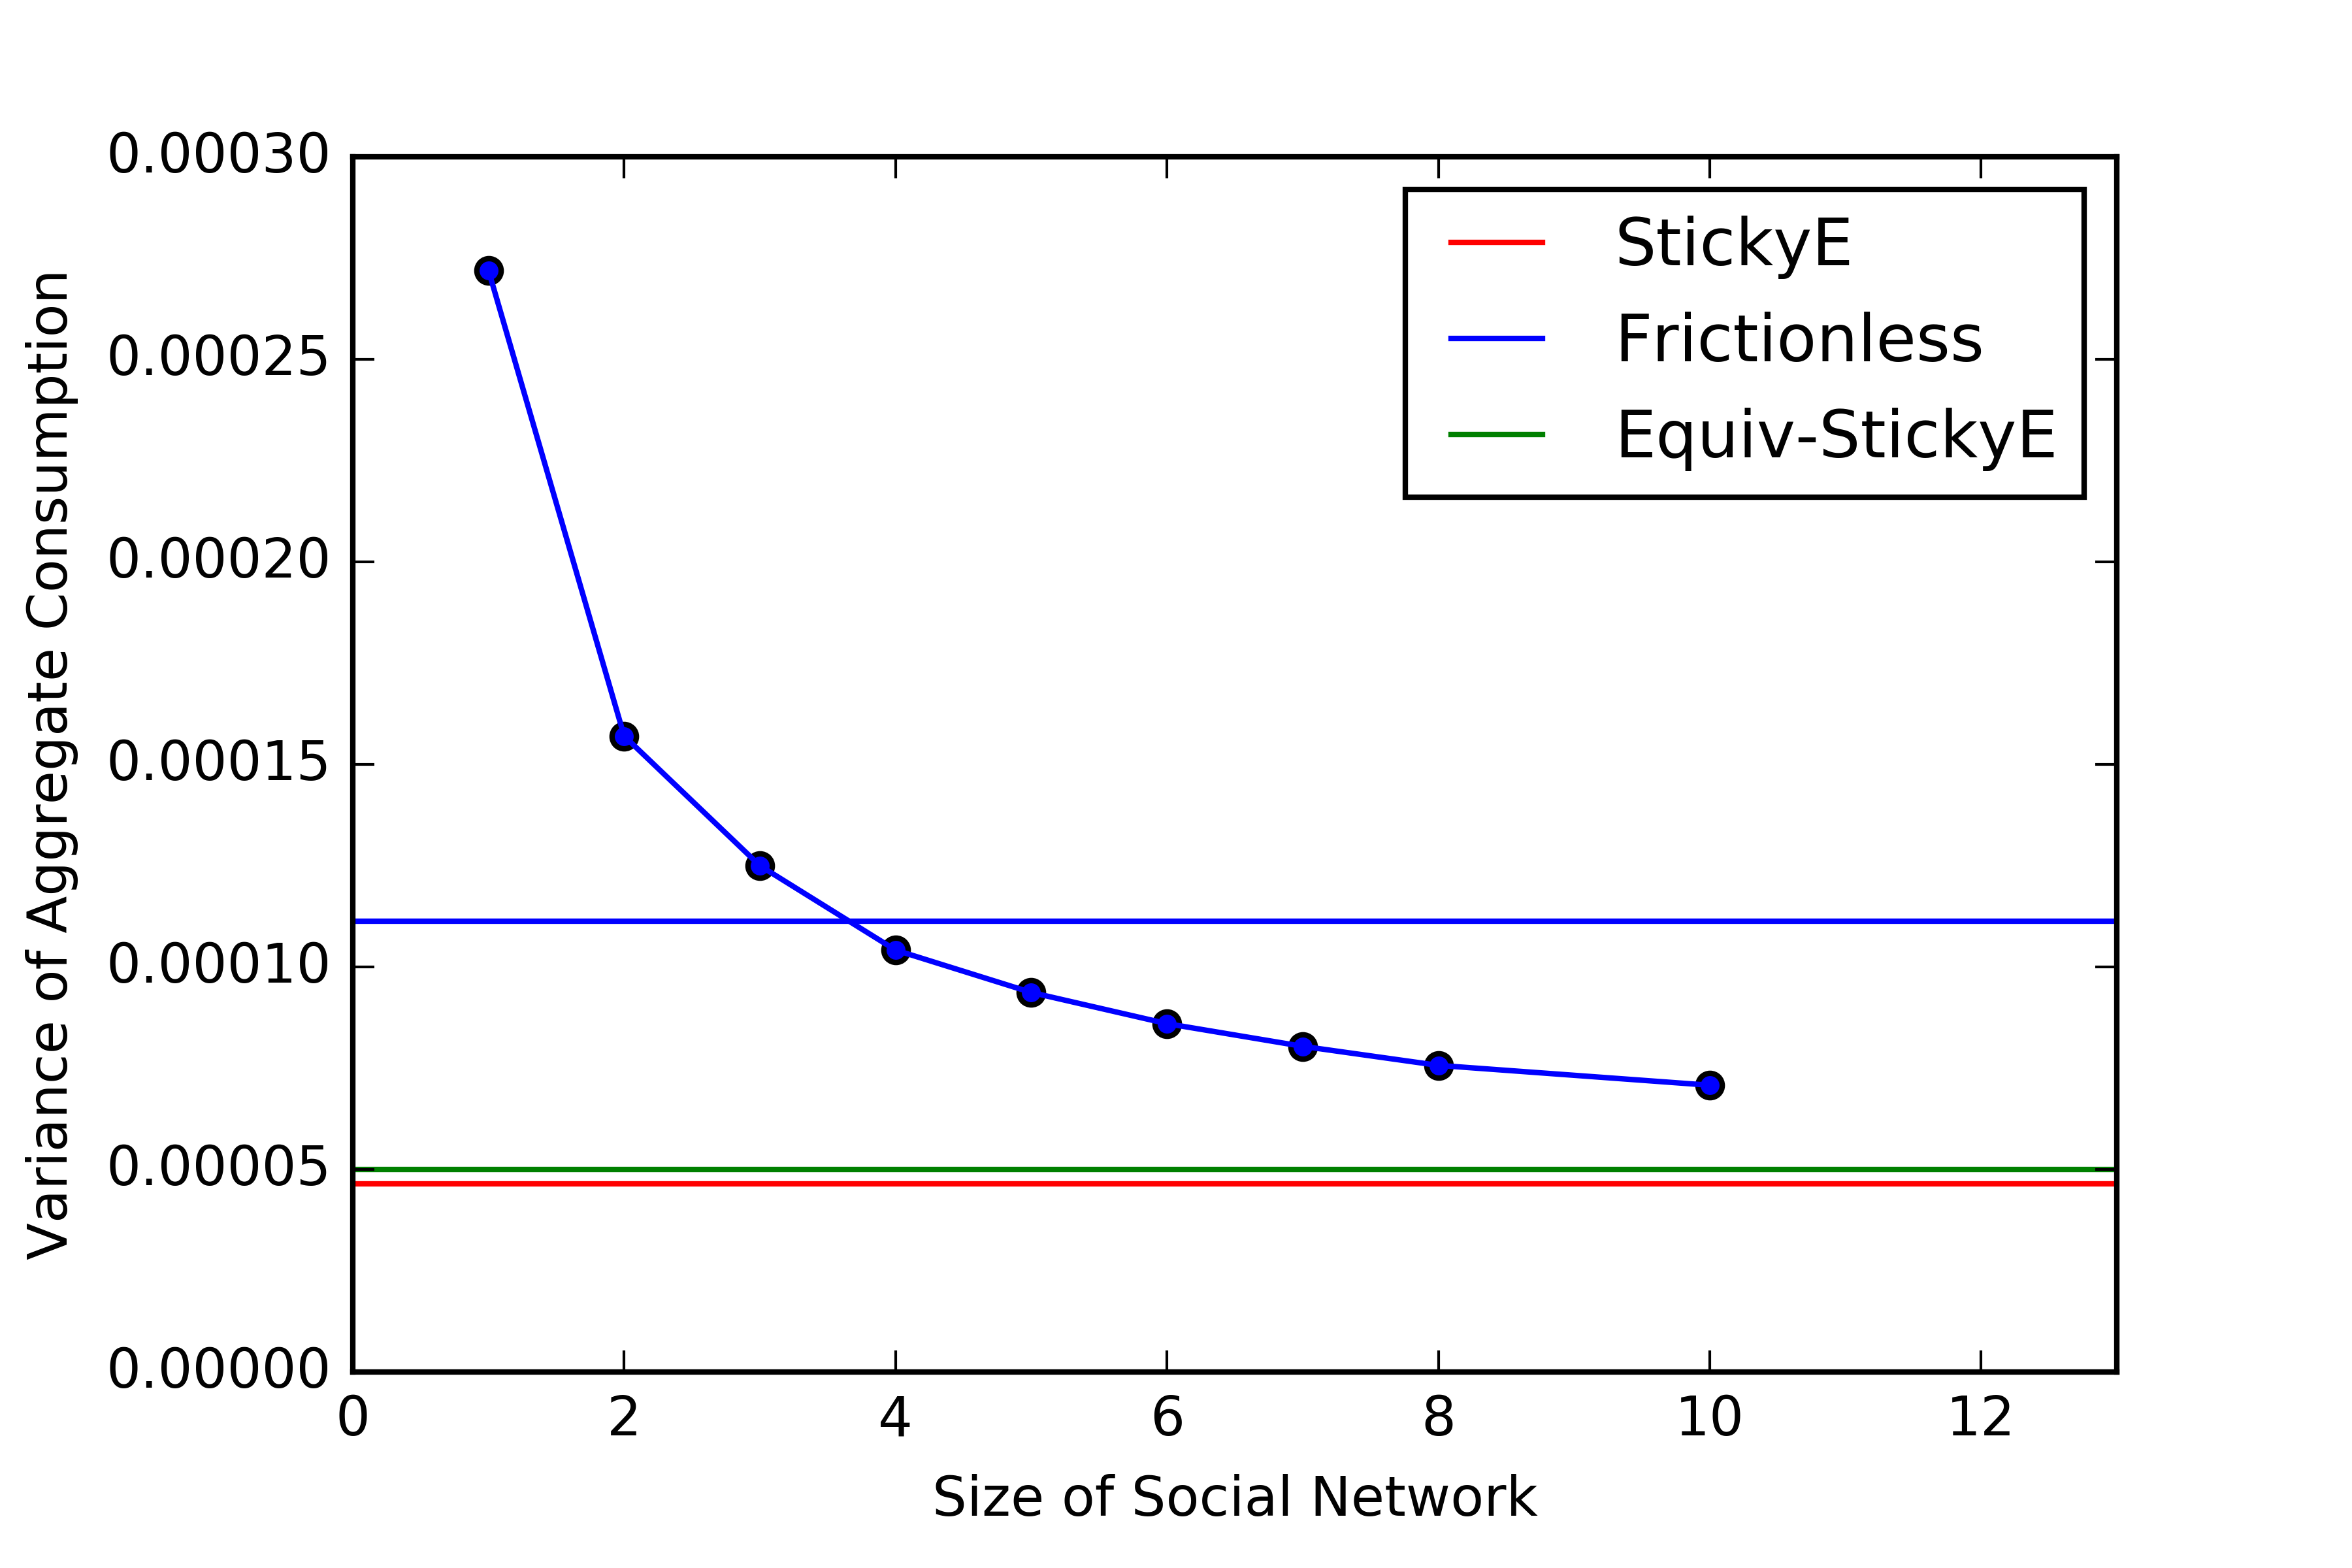
\includegraphics[scale=0.7]{p_agg.png}
	\centering
	\caption{The Variance of Aggregate Consumption for Different Size of Neighborhood}
	\label{figure:AggModel}
\end{figure}
So the aggregate consumption is affected by both idiosyncratic shocks and aggregate shocks. Because the variance of idiosyncratic shocks is much larger than the variance of aggregate shocks, the variance of aggregate consumption is higher in the model with social learning. I compute the $\text{cov}\left(\tilde{P}_{t,i},\text{ }p_{t,i}\right)$ for $n\leq4$, the result shows that as the size of neighborhood $n$ increases, the effect of ``group think'' diminishes. As $n\rightarrow+\infty$, the variance of aggregate consumption converges to a model where there is no ``group think'' effect, i.e. $\text{cov}\left(\tilde{P}_{t,i},\text{ }p_{t,i}\right)=0$. In this extreme case, the household individual productivity factor $p_{t,i}$ is not correlated with his perception of aggregate productivity $\tilde{P}_{t,i}$. 
In Section 2, we showed that allowing consumers to update their perceptions through social gathering reduces the sluggishness of aggregate consumption, quantitatively, the model that allows consumer to socially update their perceptions produces the same aggregate consumption dynamic as an equivalent sticky expectation model with modified probability of updating $\tilde{\Pi}=\frac{\Pi}{1-\left(1-\Pi\right)S}$ .  We can see from Figure \ref{figure:AggModel} that the variance of aggregate consumption from the simulation is higher than the result from the equivalent sticky expectation model. This is due to the ``group think'' effect we discussed above. In the extreme case when $n\rightarrow+\infty$, household idiosyncratic shocks cancel out each other, the aggregate consumption is not affected by idiosyncratic shocks. \par
In the last column of Table 2, I present the equilibrium statistics from the model when $n=10$. Due to the limit of time and computing power, $n=10$ is the largest neighborhood I can compute. Even though there is still distance between the result from the equivalent sticky expectation model and the social leaning model when $n=10$. I believe the result will eventually converge as $n$ increase. As a robustness check, in Appendix B.1, I provide an alternative way to show that the intuition we derived in Section 2 holds in the model with realistic settings.
\subsection{Individual Consumption}
Figure \ref{figure:IndModel} shows the variance of individual consumption ($\sigma^2_{\pmb{\mathrm{c}}}$) when the size of neighborhood changes. We can see that the variance of individual consumption is the same for the frictionless model, the original sticky expectation model, and the equivalent sticky expectation model. This is because, in these models, the volatility of consumption is caused by the volatility of perceived individual productivity $\sigma^{2}_{\tilde{\pmb{p}}_{t,i}}$. According to the calibration we described in Section 4, the variance of idiosyncratic shocks is much larger than the variance of aggregate shocks. The volatility of individual consumption is mostly caused by the volatility of the individual productivity factor $\sigma^2_{p_{t,i}}$. In these models, the consumer can correctly observe the idiosyncratic shocks. Even though the non-updating household in the sticky expectation model do not observe the aggregate shock, the difference in the variance of perceived productivity is very small. The level of variance of the individual consumption is approximately the same in the frictionless model and the original sticky expectation model.
\begin{eqnarray} \label{Result:Ind1}
\sigma^{2}_{\tilde{\pmb{p}}_{t,i}|frictionless}\approx\sigma^{2}_{\tilde{\pmb{p}}_{t,i}|stickyE}\approx\sigma^2_{p_{t,i}}
\end{eqnarray}
However, the variance of individual consumption in the model with social learning is significantly larger than the result from the frictionless model and the original sticky expectation model. It is because for the socially updating household, his perception of aggregate productivity $\tilde{P}_{t,i}$ contains his neighbors' individual productivity factor $p_{t,i+j}$. The variance of his perceived aggregate productivity $\tilde{P}_{t,i}$ is comparable with the variance of his individual productivity factor $p_{t,i}$. Because
\begin{equation*}
\sigma^{2}_{\tilde{\pmb{p}}_{t,i}|social}=\text{Var}(p_{t,i}\tilde{P}_{t,i})
\end{equation*}
In Section 5.1, we showed that the $p_{t,i}$ and $\tilde{P}_{t,i}$ are positively correlated in the social learning model. As a result: $\sigma^{2}_{\tilde{\pmb{p}}_{t,i}|social}>\text{Var}(\sigma^2_{p_{t,i}})$. So
\begin{equation}\label{Result:Ind2}
\sigma^{2}_{\pmb{c}|social}>\sigma^{2}_{\pmb{c}|frictionless}\approx\sigma^{2}_{\pmb{c}|stickyE}
\end{equation}
When the size of neighborhood $n$ increases, for a socially updating household, his neighbors' idiosyncratic shocks cancel out each other, and the variance of his perception of aggregate productivity becomes smaller. The variance of individual consumption in the social learning model converges to the result from the equivalent sticky expectation model when $n\rightarrow+\infty$.
\begin{figure}[h]
	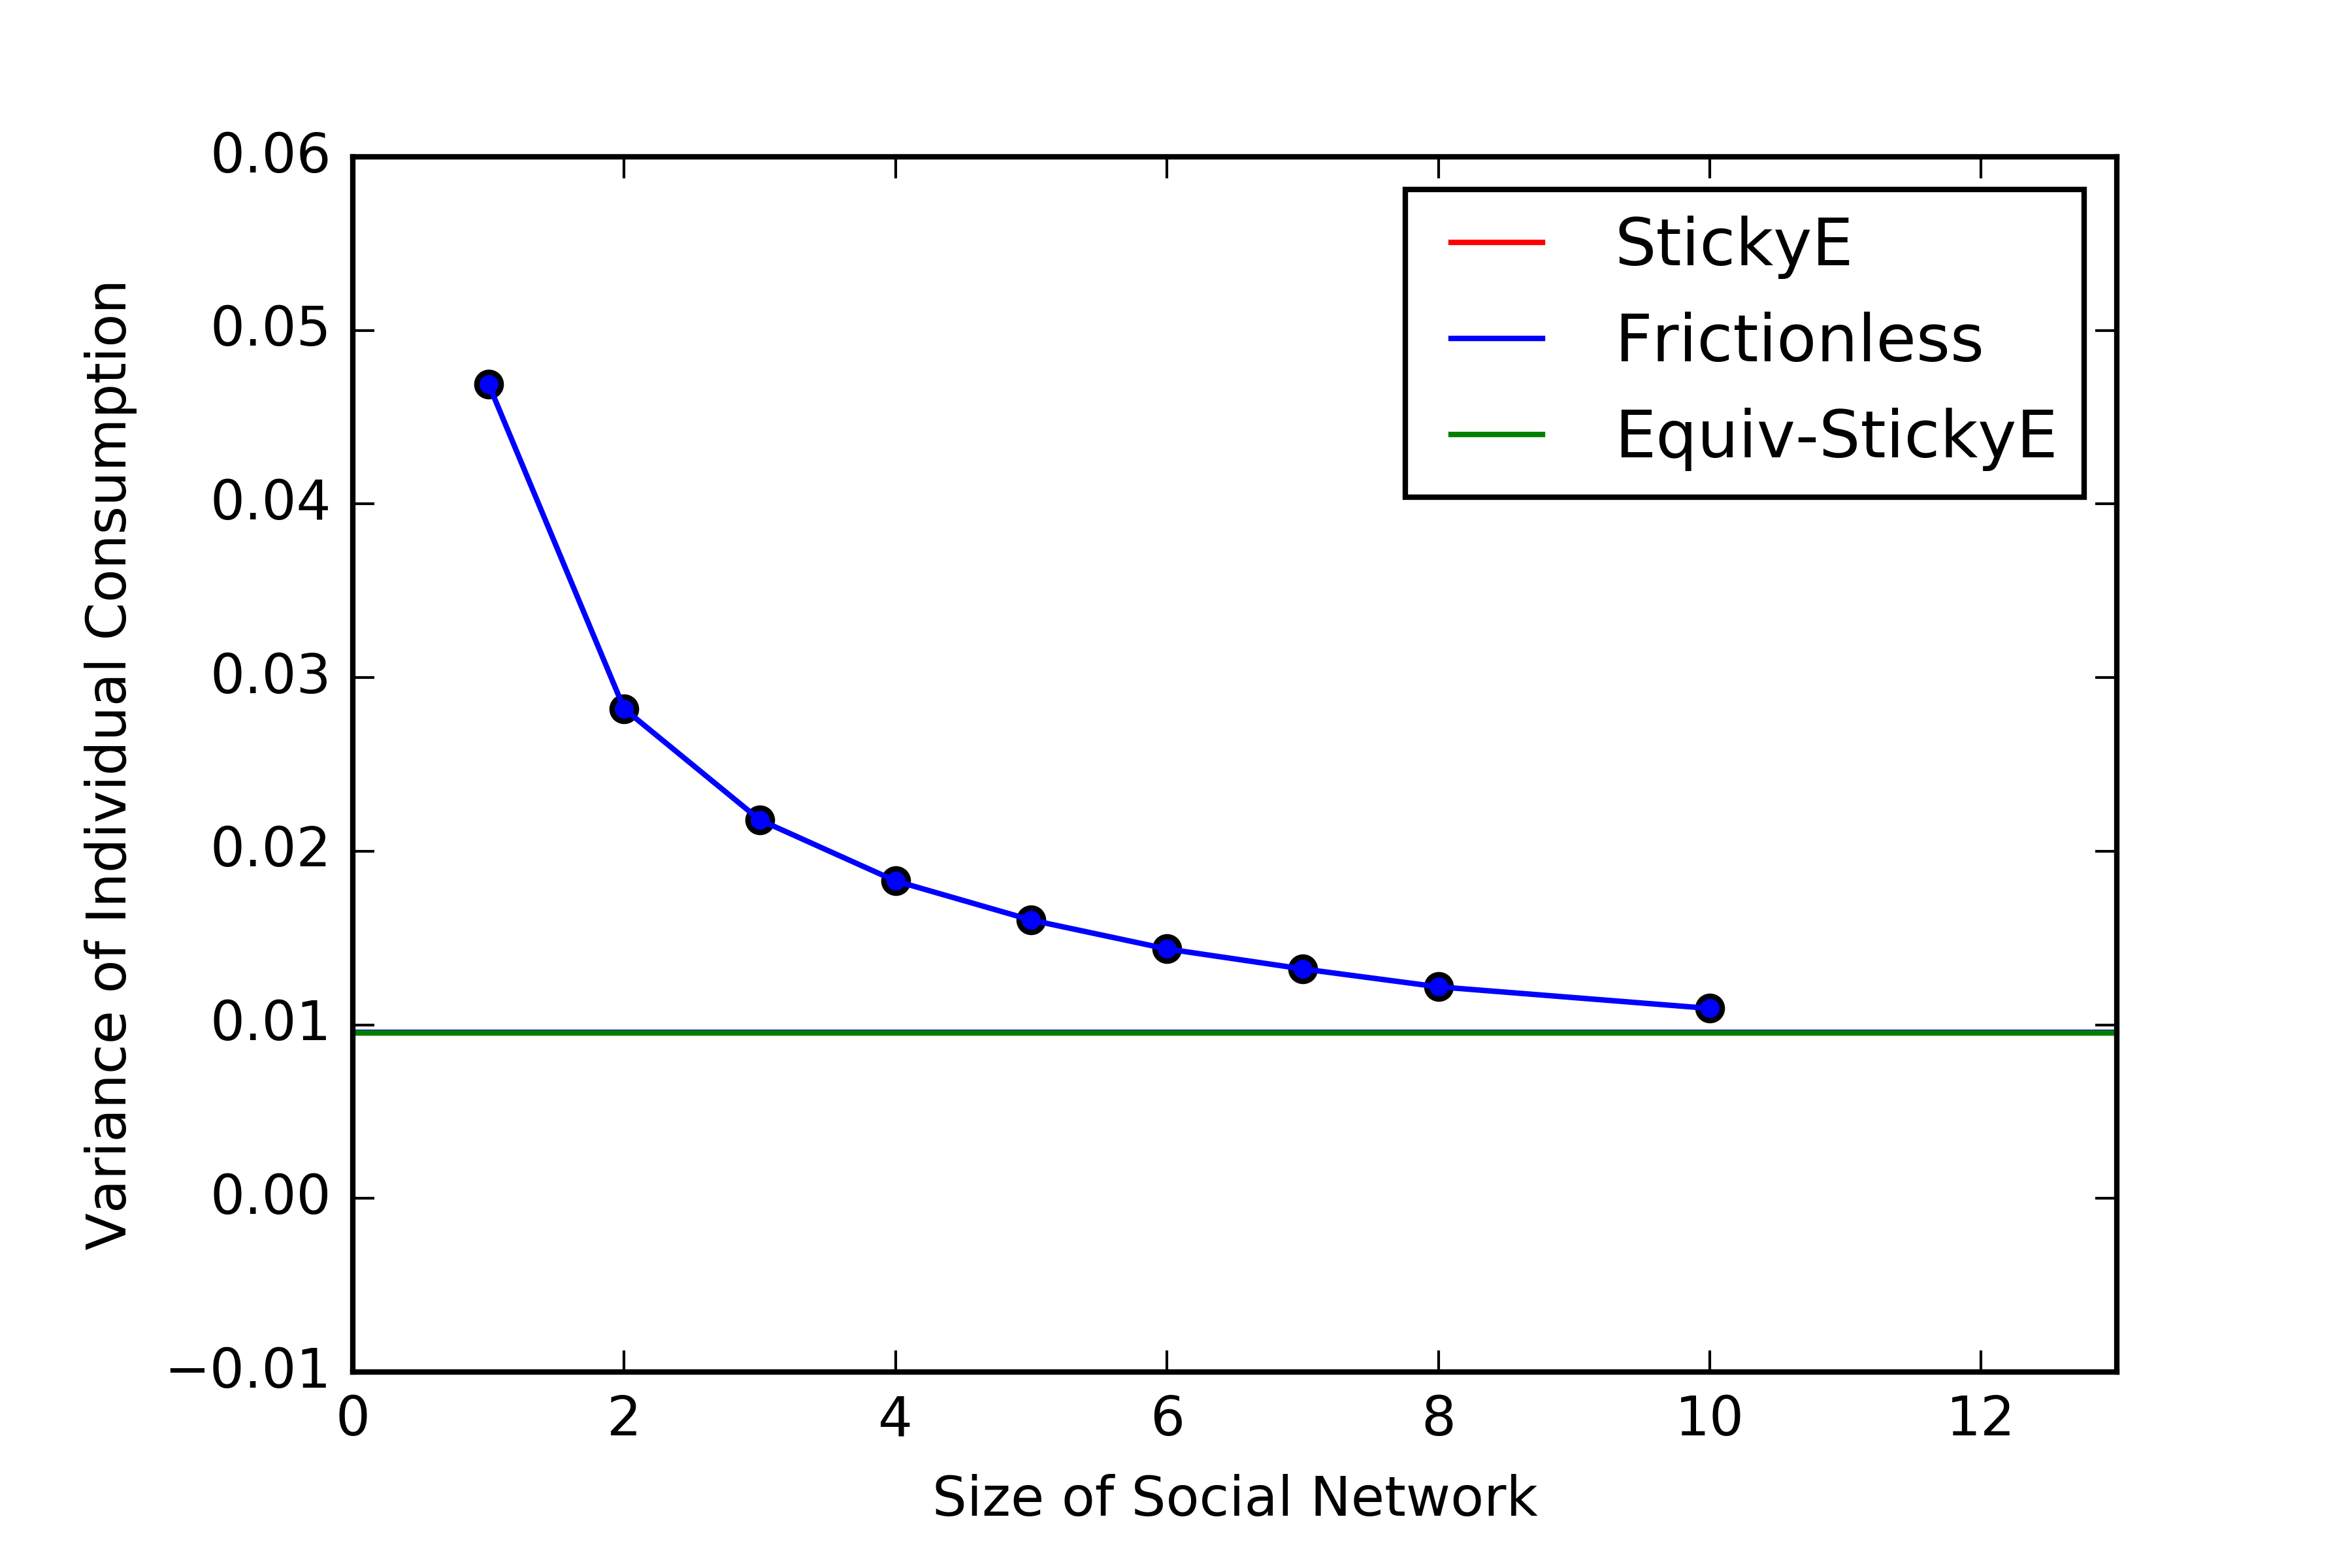
\includegraphics[scale=0.7]{p_ind.png}
	\centering
	\caption{The Variance of Individual Consumption for Different Size of Neighborhood. Here the variance is calculated across time and individuals}
	\label{figure:IndModel}
\end{figure}
\section{Conclusion}
There is extensive literature that studies how an individual's consumption is influenced by other members from his social network. The possible contribution of such influence to the boom and bust cycle attracted more attention after the Financial Crisis. (\cite{FaultLines}, \cite{IMFReport}, \cite{Trickle})
\par
Differing from previous literature that incorporate relative consumption into the household's utility function, the model from this paper provides an alternative way for an individual's consumption decision to be influenced by other people in the society. Building upon the sticky expectation framework where consumers do not always observe the true aggregate states, the model in this paper allows consumers to form their expectations based on his neighbors' perceptions of the aggregate state. Through this channel, perceptions of neighbors of one individual can affect that individual's consumption decision by affecting his information set, which affects his expectation of future income.
\par
Since the socially updating household can not distinguish his neighbor's individual productivity factor from the neighbor's perceived aggregate productivity, the socially updating household's perception of aggregate productivity is affected by his neighbors' idiosyncratic shocks. Because idiosyncratic shocks are significantly more volatile than aggregate shocks, compared to the original sticky expectation model where perceptions of aggregate states are only affected by aggregate shocks, the model with socially formed expectation produces larger variances for individual consumption and aggregate consumption.
\par
The higher variance of aggregate consumption is the result of two factors. First, allowing consumers to socially update their perceptions gives them another channel to update their information, reducing the sluggishness of aggregate consumption. Second, in the case that a household and some of his neighbors both socially update their perceptions, the household perception of aggregate productivity will be positively correlated with his own individual productivity factors. As a result of this ``group think'' effect, aggregate consumption are subject to idiosyncratic shocks because the idiosyncratic shocks do not cancel out each other in aggregation. Because the variance of idiosyncratic shocks are much larger than the variance of aggregate shocks, the social learning increases the variance of aggregate consumption. As the size of neighborhood increases, the ``group think'' effect disappears, the model with socially formed expectations converges to an equivalent sticky expectation model with a modified probability of updating to the true aggregate state.
\par
One possible weakness of the model is that it contradicts the original purpose of the sticky expectation model: to explain the sluggishness of the consumption growth. However, we can see that under reasonable calibration, the model with social learning is equivalent with (or converges to) a sticky expectation model where $\tilde{\Pi}\approx0.29$. This number lies in the range of empirical estimations. This shows that the model with social learning has the potential to incorporate the impact of the social network while still matching the quarterly consumption dynamics.
\par
This paper intends to be a small step towards understanding the influence of the social network on aggregate consumption dynamics. One interesting extension for future research could be to group agents into neighborhoods based on their income or education level instead of randomly assigning them, as was the case in this model. Such residential segregation is documented in literature. \cite[]{ResidentialEvidence} Learning from neighbors may explain why people from different income backgrounds have different views of the macroeconomy.
\newpage
\begin{table}
	\centering
	\caption{Calibration}
	%\setlength\arrayrulewidth{2pt}
	\begin{tabular*}{\textwidth}{c @{\extracolsep{\fill}} lll}\noalign{\hrule height 2pt}
		\bfseries Preference Parameter~ & \bfseries ~ & \bfseries ~
		\csvreader[head to column names]{Pref.csv}{}
		{\\[5 pt] \csvcolii&\csvcoliii&\csvcoli}
		\\\hline
		\bfseries Idiosyncratic Shock Parameters~ & \bfseries ~ & \bfseries ~
		\csvreader[head to column names]{Idio.csv}{}
		{\\[5 pt] \csvcolii&\csvcoliii&\csvcoli}
		\\\hline
		\bfseries Macroeconomic Parameter~ & \bfseries ~ & \bfseries ~
		\csvreader[head to column names]{Macro.csv}{}
		{\\[5 pt] \csvcolii&\csvcoliii&\csvcoli}
		\\\noalign{\hrule height 2pt}
	\end{tabular*}
\end{table}
\clearpage
\begin{table}
	\centering
	\caption{Equilibrium Statistics}
	\label{tab:Uncert}
	\begin{center}
		\begin{tabular}{ l c c c c}\noalign{\hrule height 2pt}
			~ & Frictionless & StickyE & Equiv-StickyE & Social $(n=10)$\\
			\hline
			Means\\ 
			\hspace{6mm}$\mathrm{A}$ & 7.44 & 7.43 & 7.43 & 8.81\\
			\hspace{6mm}$\mathrm{C}$ & 2.71 & 2.71 & 2.71 & 2.73\\
			\hline
			Standard Deviation\\
			\hspace{3mm}Aggregate Time Serie\\
			\hspace{6mm}$\text{log }\mathrm{A}$ & 0.332 & 0.320 & 0.322 & 0.351\\
			\hspace{6mm}$\Delta \text{log }\mathrm{C}$ & 0.0106 & 0.0068 & 0.0070 & 0.008\\
			\hspace{6mm}$\Delta \text{log }\mathrm{Y}$ & 0.015 & 0.015 & 0.015 & 0.015\\
			\hspace{3mm}Individual Cross Sectional\\
			\hspace{6mm}$\text{log }p$ & 0.790 & 0.790 & 0.790& 0.790\\
			\hspace{6mm}$\Delta \text{log }\pmb{\mathrm{c}}$ & 0.098 & 0.098 & 0.098 & 0.138\\									
			\hline
		\end{tabular}
		\\
	\end{center}
	\begin{tablenotes}
		\small
		\item \textbf{Note}: Equiv-StickyE is the sticky expectation model with the modified probability of updating $\tilde{\Pi}=\frac{\Pi}{1-\left(1-\Pi\right)S}\geq\Pi$.
	\end{tablenotes}
\end{table}
\clearpage
% Remove or comment out the next two lines if you are not using bibtex.
%%\bibliographystyle{aea}
%%\bibliography{BibFile}
% The appendix command is issued once, prior to all appendices, if any.
\bibliographystyle{plainnat}

\bibliography{Reference}
\clearpage
\appendix
\section{Derivation}
\subsection{Aggregate Consumption Dynamic in Toy Model}
This section derives the dynamic of aggregate consumption in the toy model.The aggregate consumption is a fixed fraction of total wealth: (Capital letters denote the aggregate variable)
\begin{eqnarray}
\mathrm{C}^{\pi}_{t} & = & \Pi^{-1}\int_{0}^{1}\pi_{t,i}\mathrm{c}_{t,i}\text{d}i \nonumber\\
& = & \Pi^{-1}\int_{0}^{1}\pi_{t,i}\left(\frac{\mathsf{r}}{\mathsf{R}}\mathrm{o}_{t,i}\right)\text{d}i \nonumber\\
& = & \left(\frac{\mathsf{r}}{\Pi\mathsf{R}}\right)\int_{0}^{1}\pi_{t,i}\mathrm{o}_{t,i}\text{d}i \nonumber\\
& = & \left(\frac{\mathsf{r}}{\Pi\mathsf{R}}\right)\Pi\mathrm{O}_{t} \nonumber\\
& = & \frac{\mathsf{r}}{\mathsf{R}}\mathrm{O}_{t} \nonumber
\end{eqnarray}
We can decompose the total wealth as non-human wealth and the future human wealth:
\begin{equation}
\mathrm{O}_{t}=\mathrm{B}_{t}+\left(\Theta_{t}-1\right)\mathsf{p}_{t}+\mathrm{H}_{t}
\end{equation}
Here $\mathrm{B}_{t}$ is the level of aggregate non-human asset at the beginning of period $t$, evolves according to the dynamic budget constraint.
\begin{eqnarray}
\mathrm{B}_{t+1} & = & \mathsf{R}\mathrm{A}_{t} \nonumber\\
& = & \mathsf{R}\left(\mathrm{B}_{t}+\mathrm{Y}_{t}-\mathrm{C}_{t}\right)
\end{eqnarray} 
The non-capital income $\mathrm{Y}_{t}$ evolves according to equation (\ref{Toy:Income})
\begin{eqnarray*}
	\mathrm{Y}_{t+1}=\mathsf{p}_{t+1}\Theta_{t+1}\\
	\mathrm{p}_{t+1}=\mathsf{p}_{t}\Psi_{t+1}
\end{eqnarray*}
Here $\mathrm{Y}_{t}=\mathrm{y}_{t}$ $\forall\text{ }t$ because every household has the same income process. $\mathsf{p}$ is the level of permanent income, $\Theta$ and $\Psi$ are mean $1$, i.i.d transitory and permanent shocks.  The human wealth $\mathrm{H}_{t}$ is the discounted future non-capital income
\begin{eqnarray}
\mathrm{H}_{t} & = & \mathsf{p}_{t}+\frac{\E_{t}[\mathrm{Y}_{t+1}]}{\mathsf{R}}+\frac{\E_{t}[\mathrm{Y}_{t+2}]}{\mathsf{R}^2}+\frac{\E_{t}[\mathrm{Y}_{t+3}]}{\mathsf{R}^3}+\cdots\\
& = & \mathsf{p}_{t}+\frac{\E_{t}[\mathsf{p}_{t+1}]}{\mathsf{R}}+\frac{\E_{t}[\mathsf{p}_{t+2}]}{\mathsf{R}^2}+\frac{\E_{t}[\mathsf{p}_{t+3}]}{\mathsf{R}^3}+\cdots\\
& = & \frac{\mathsf{R}}{\mathsf{r}}\mathsf{p}_{t}
\end{eqnarray}
Given the income process, for each consumer, his total wealth evolves according to:
\begin{eqnarray*}
	\mathsf{o}_{t+1} & = & \mathrm{b}_{t+1}+\left(\Theta_{t+1}-1\right)\mathsf{p}_{t+1}+\mathrm{H}_{t+1}\\
	& = & \mathsf{R}\left(\mathrm{b}_{t}+\mathrm{y}_{t}-\mathrm{c}_{t}\right)+\left(\Theta_{t+1}-1\right)\Psi_{t+1}\mathsf{p}_{t}+\frac{\mathsf{R}}{\mathsf{r}}\mathsf{p}_{t}\Psi_{t+1}\\
	& = & \mathsf{R}\left(\mathsf{o}_{t}-\mathrm{c}_{t}\right)+\underbrace{\left(\Theta_{t+1}-1\right)\Psi_{t+1}\mathsf{p}_{t}+\frac{\mathsf{R}}{\mathsf{r}}\mathsf{p}_{t}\left(\Psi_{t+1}-1\right)}_{=\xi_{t+1}}
\end{eqnarray*}
which is consistent with dynamic budget constraint (\ref{Toy:DBC}) of the model in section 2. When there is no informational friction, $\mathrm{c}_{t}=\frac{\mathsf{r}}{\mathsf{R}}\mathrm{o}_{t}$. The total wealth follows a random walk:
\begin{eqnarray*}
	\mathsf{o}_{t+1}& = & \mathsf{R}\left[\mathrm{b}_{t}+\mathrm{y}_{t}-\frac{r}{R}\left(\mathrm{b}_{t}+\left(\Theta_{t}-1\right)\mathsf{p}_{t}+\mathrm{H}_{t}\right)\right]+\left(\Theta_{t+1}-1\right)\Psi_{t+1}\mathsf{p}_{t}+\frac{\mathsf{R}}{\mathsf{r}}\mathsf{p}_{t}\Psi_{t+1}\\
	& = &
	\mathrm{b}_{t}+\left(\Theta_{t}-1\right)\mathsf{p}_{t}+\frac{\mathsf{R}}{\mathsf{r}}\mathsf{p}_{t}+\xi_{t+1}\\
	& = & \mathrm{o}_{t}+\xi_{t+1}\\
\end{eqnarray*}
In the sticky expectation model, for consumers who observe the true state, their average consumption level is:
\begin{eqnarray} \label{A1: AggC}
\mathrm{C}^{\pi}_{t+1} & = & \frac{\mathsf{r}}{\mathsf{R}}\left(\mathrm{B}_{t+1}+\left(\Theta_{t+1}-1\right)\mathsf{p}_{t+1}+\mathrm{H}_{t+1}\right) \\
& = & \frac{\mathsf{r}}{\mathsf{R}}\left[\mathsf{R}\left(\mathrm{B}_{t}+\mathrm{Y}_{t}-\mathrm{C}_{t}\right)+\left(\Theta_{t+1}-1\right)\mathsf{p}_{t+1}+\mathrm{H}_{t+1}\right] \nonumber\\
& = & \left[\left(\mathrm{B}_{t}+\Theta_{t}\mathsf{p}_{t}-\mathrm{C}_{t}\right)\mathsf{R}+\left(\Theta_{t+1}-1\right)\mathsf{p}_{t}\right]\frac{\mathsf{r}}{\mathsf{R}}+\left(\Theta_{t+1}-1\right)\mathsf{p}_{t}\left(\Psi_{t+1}-1\right)\frac{\mathsf{r}}{\mathsf{R}}+\mathsf{p}_{t}\Psi_{t+1} \nonumber
\end{eqnarray}
Let $\hat{\Theta}_{t+1}=\Theta_{t+1}-1$, $\hat{\Psi}_{t+1}=\Psi_{t+1}-1$, and $\kappa=\frac{\mathsf{r}}{\mathsf{R}}$. Equation (\ref{A1: AggC}) can be written as:
\begin{eqnarray}
\mathrm{C}^{\pi}_{t+1} & = & \left[\left(\mathrm{B}_{t}+\Theta_{t}\mathsf{p}_{t}-\mathrm{C}_{t}\right)\mathsf{R}+\hat{\Theta}_{t+1}\mathsf{p}_{t}\right]\kappa+\hat{\Theta}_{t+1}\hat{\Psi}_{t+1}\kappa\mathsf{p}_{t}+\mathsf{p}_{t}+\hat{\Psi}_{t+1}\mathsf{p}_{t} \nonumber \\
& = & \underbrace{\left[\left(\mathrm{B}_{t}+\Theta_{t}\mathsf{p}_{t}-\mathrm{C}^{\pi}_{t}\right)\mathsf{R}+\hat{\Theta}_{t+1}\mathsf{p}_{t}\right]\kappa+\mathsf{p}_{t}}_{=\E_{t}[\mathrm{C}_{t+1|\tau_{t+1}=t}]+\kappa\hat{\Theta}_{t+1}}+\left(\hat{\Psi}_{t+1}+\hat{\Theta}_{t+1}\hat{\Psi}_{t+1}\kappa\right)\mathsf{p}_{t}+\mathsf{R}\kappa\left(\mathrm{C}^{\pi}_{t}-\mathrm{C}_{t}\right) \nonumber
\end{eqnarray}
Here $\mathrm{C}^{\pi}_{t}$ represents the average consumption in time period $t$ of households who observe the true aggregate states in period $t$. $\mathrm{C}_{t+1|\tau_{t+1}=t}$ represents the average consumption in time period $t+1$ of households who observed the news in period $t$ but not in period $t+1$. Because the consumption of fully informed consumers follows a random walk process, $\E_{t}[\mathrm{C}_{t+1|\tau_{t+1}=t}]=\mathrm{C}^{\pi}_{t}$, which means:
\begin{eqnarray} \label{A1:AfterEx}
\mathrm{C}^{\pi}_{t+1} & = & \mathrm{C}^{\pi}_{t}+\mathsf{R}\kappa\left(\mathrm{C}^{\pi}_{t}-\mathrm{C}_{t}\right)+\left(\hat{\Psi}_{t+1}+\hat{\Theta}_{t+1}\hat{\Psi}_{t+1}\kappa\right)\mathsf{p}_{t}
\end{eqnarray}
From equation (\ref{Toy:StickyE}), we know:
\begin{eqnarray}
\mathrm{C}_{t+1} & = & \Pi\mathrm{C}^{\pi}_{t+1}+\left(1-\Pi\right)\mathrm{C}_{t} \label{A1:sub1}\\
\mathrm{C}_{t} & = & \Pi\mathrm{C}^{\pi}_{t}+\left(1-\Pi\right)\mathrm{C}_{t-1}\label{A1:sub2}
\end{eqnarray}
Subtracting equation (\ref{A1:sub2}) from (\ref{A1:sub1}), we have:
\begin{eqnarray} \label{A1:DeltaC}
\mathrm{C}^{\pi}_{t+1}-\mathrm{C}^{\pi}_{t} & = & \frac{\Delta\mathrm{C}_{t+1}-\left(1-\Pi\right)\Delta\mathrm{C}_{t}}{\Pi}
\end{eqnarray}
We can derive the dynamic of aggregate consumption by combining equation (\ref{A1:AfterEx}) and (\ref{A1:DeltaC}):
\begin{eqnarray} \label{A1:Final}
\Delta\mathrm{C}_{t+1} & = & \mathsf{R}\left(1-\Pi\right)\Delta\mathrm{C}_{t}+\underbrace{\left(\hat{\Psi}_{t+1}+\kappa\hat{\Theta}_{t+1}\Psi_{t+1}\right)\Pi}_{=\epsilon_{t+1}}
\end{eqnarray}
\subsection{The Definition of Neighborhood for A continuum of Agents}
In the main text, I introduce the concept of the neighborhood in the context when the number of agents is countable. This is true for a computer simulation. However, in the theoretical model setting in Section 3, agents occupy a continuum of positions. In this section, I define the neighborhood of the agent when there is a continuum of agents in the economy. The mass of agents is normalized to one. Follows the setting in section 2.2 in the main text, all agents sit in a circle. In this case, we can define the size of the neighborhood $n \in (0,1)$, which measures the distance from one agent and his farthest neighbor on the circle. For a household $i$, his neighbors are $\{\text{agent x}|\text{ }\forall x\in [i-n,i)\cup(i,i+n]\}$. In this case, the continuous version of equation (\ref{Toy:SocialUpdating}) will be:
\begin{eqnarray}
\tilde{\mathsf{p}}_{t,i}=\frac{1}{2n}\int_{-n}^{n}\tilde{\mathsf{p}}_{t,i+j}\text{d}j\text{    }j\neq 0
\end{eqnarray}
\par
In Section 3.3, I also discussed the updating mechanism by using the example when the number of agent is countable, in the case when there is a continuum of agents, equation $\ref{eq:SocialUpdateP}$ becomes:
\begin{eqnarray}
\tilde{P}_{t+1,i} = \frac{1}{2n}\left[\int_{-n}^{n}p_{t+1,i+j}\tilde{P}_{t+1,i+j}\text{d}j\right]
\end{eqnarray}
In the more realistic model that was introduced in section 3, the socially updating household $i$ randomly chooses one of his neighbor's perceived growth rate as his perception of the growth rate. In the case when there is a continuum of agents, the index variable of the neighbor that was going to be chosen by the household $i$ is uniformly distributed in household $i$'s neighborhood:
\begin{eqnarray}
\text{ Prob}(\tilde{\Phi}_{t,i}=\tilde{\Phi}_{t,i+j})=\frac{1}{2n}\text{ }\forall\text{ }-n\leq j\leq n\text{, }j\neq 0
\end{eqnarray}
\section{Additional Results}
\subsection{Limit Case}
An alternative way to show that the intuition from Section 2 carries to a model with CRRA utility and idiosyncratic income trajectories is to compute a model where the socially updating household sets his perception of aggregate productivity as the average of his neighbors' perceived aggregate productivities:
\begin{eqnarray} \label{B1}
\tilde{P}_{t,i}& = & \frac{1}{2n}\left[\sum_{j\neq0,j=-n}^{n}\tilde{P}_{t,i+j}\right]
\end{eqnarray}
Here the perception of the socially updating household does not depend on his neighbors' individual productivity factor (each person's actual income still depends on his own individual productivity factor), the rest of the model is the same as we described in Section 3. (I refer this model as Limit-Case model)
\begin{figure}[h]
	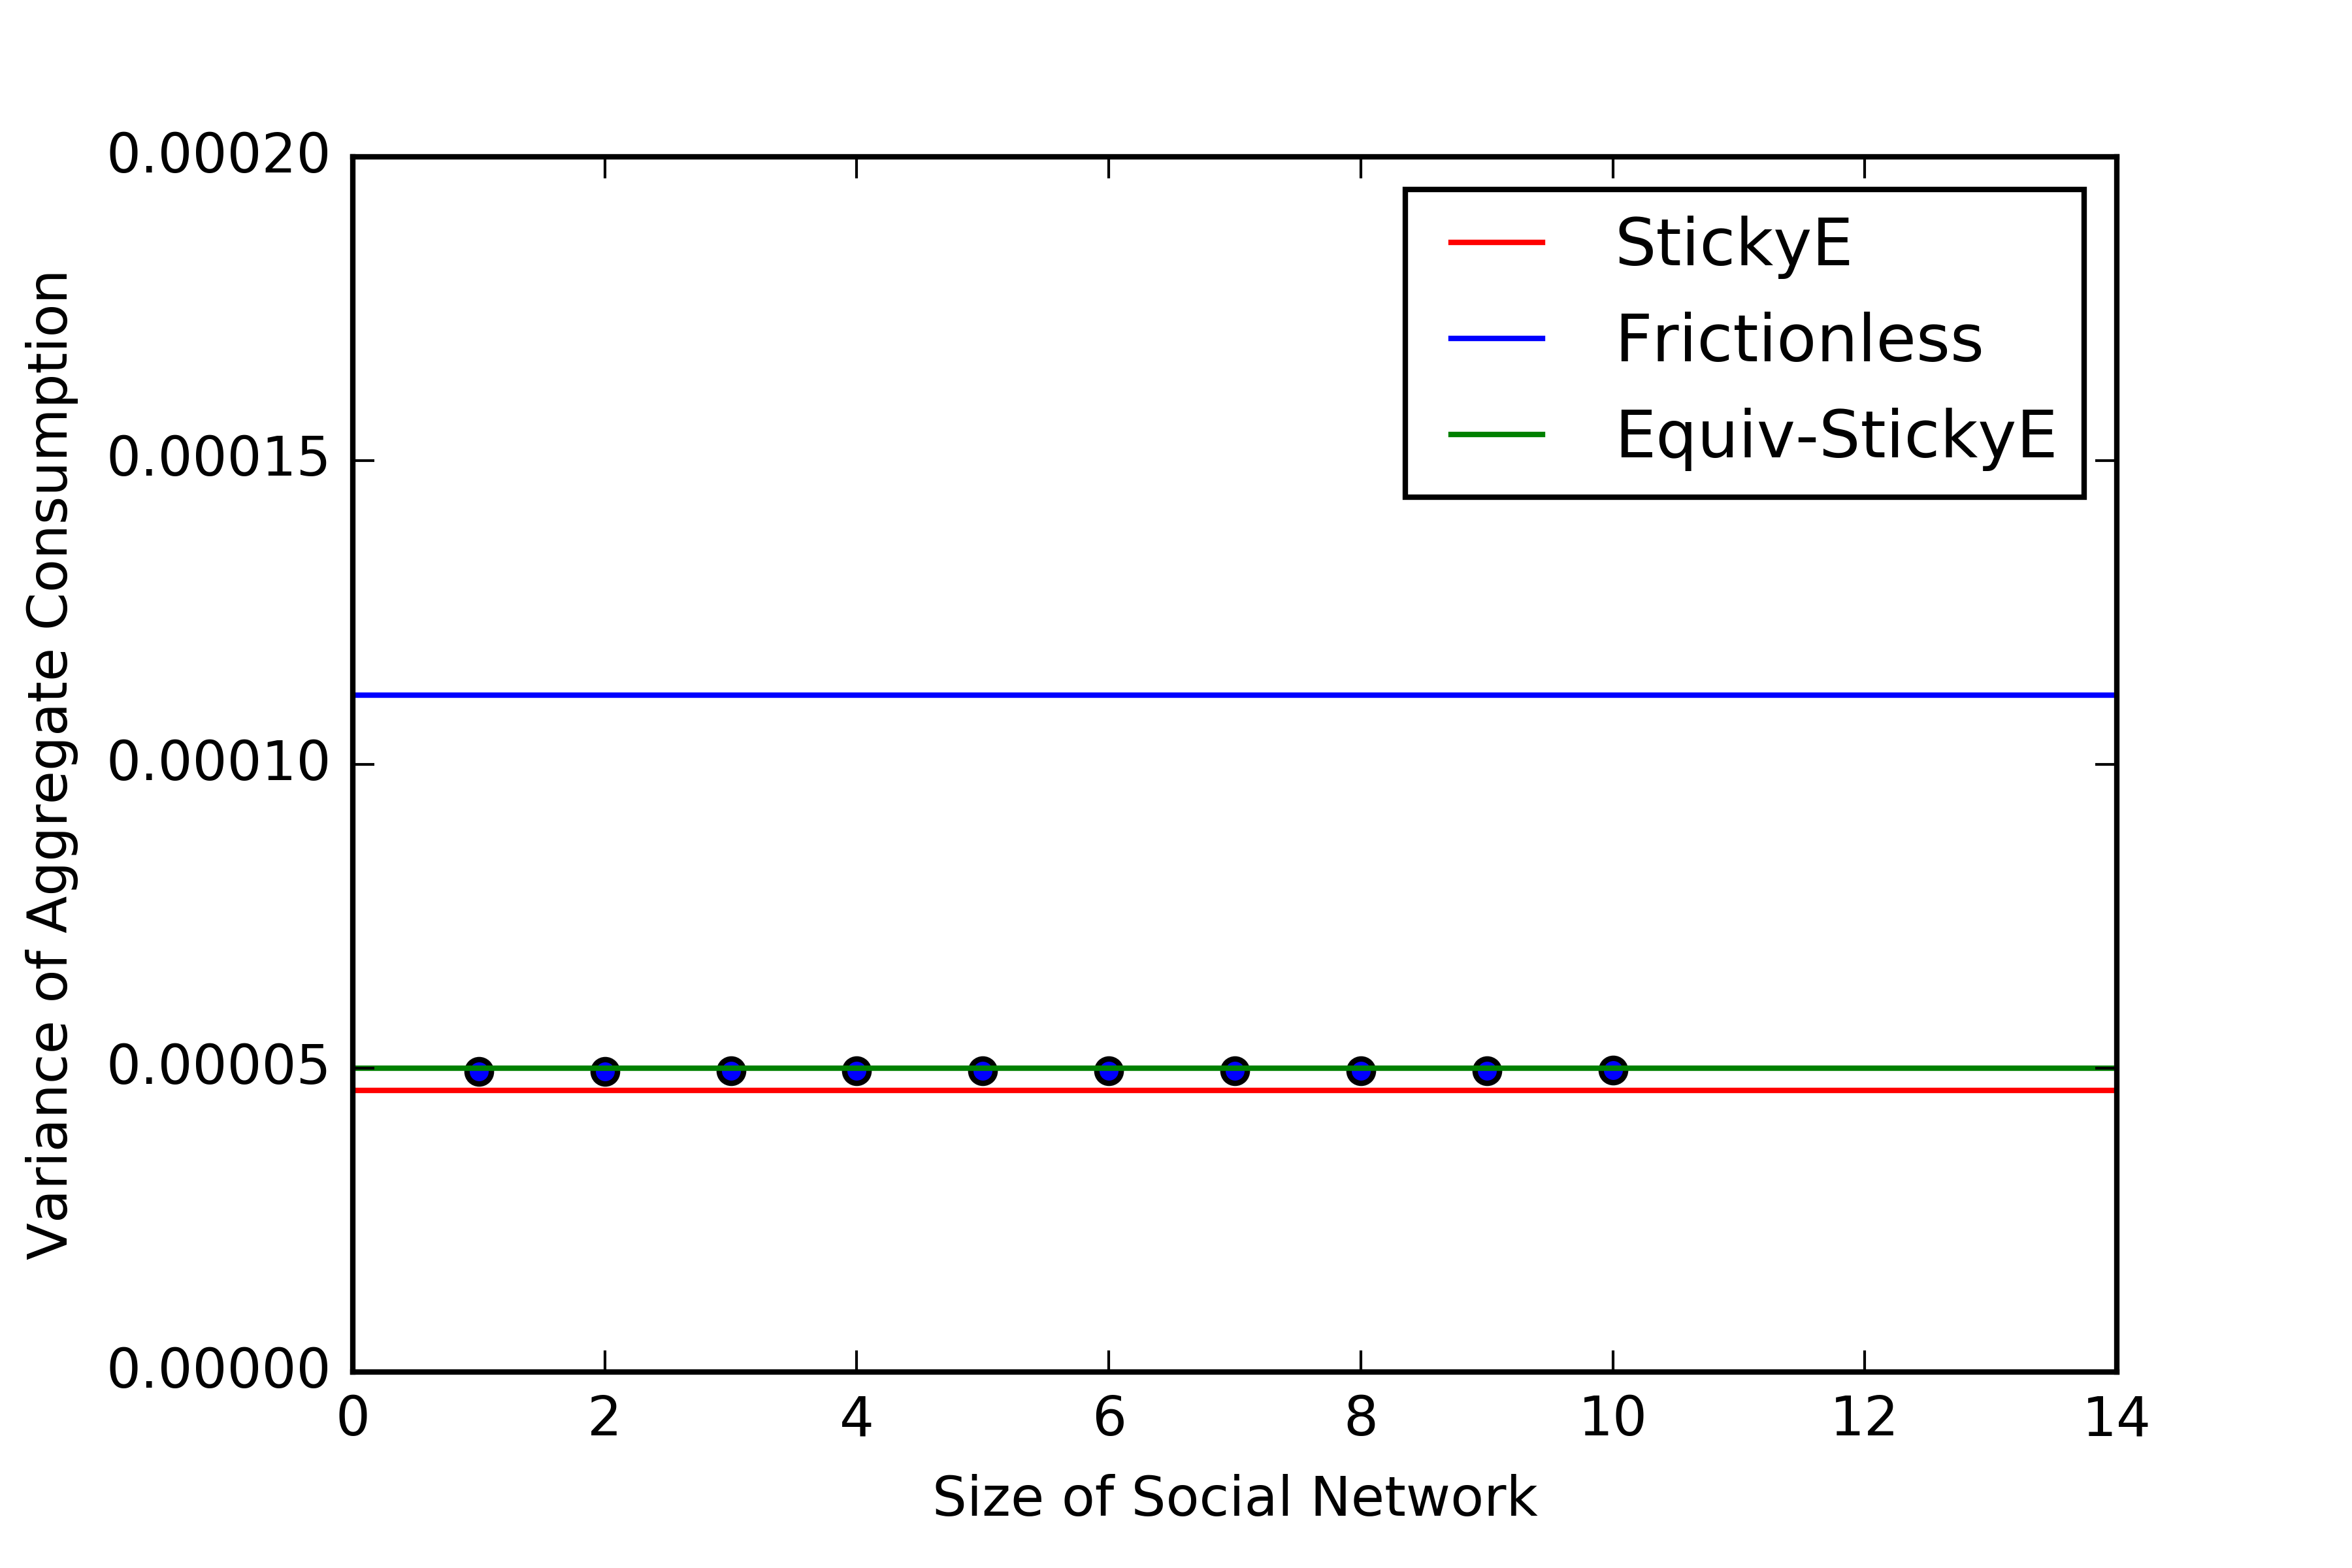
\includegraphics[scale=0.7]{Pcvd_Agg.png}
	\centering
	\caption{The Variance of Aggregate Consumption for Different Size of Neighborhood. Here the socially updating household forms his perception of aggregate productivity according to equation (\ref{B1})}
	\label{figure:AggEquiv}
\end{figure}
\par
Figure \ref{figure:AggEquiv} presents the variance of aggregate consumption from the Limit-Case model and the equivalent sticky expectation model where the probability of updating to the news is $\tilde{\Pi}$. We can see that two models yield the same variance of aggregate consumption, and $\sigma^{2}_{\Delta\mathrm{C}}$ does not change when the size of neighborhood $n$ changes.  
\end{document}

